% !TeX root = ../../Book3.tex
% 纲要标题：## 第8章　Ricci 曲率、体积比较与基本群
% 纲要位置：几何学计划纲要.md，第 2393 行。
% 正文状态：初稿；尚未正式审核。

% 纲要内容开始
% 
% > 本章目标与证明范围：完整建立直径和体积比较及其覆盖应用。Cheeger–Gromoll 分裂的证明移到已具备弱最大值和 Bochner 工具的位置，不在这里隐藏分析先修。
% 
% 纲要内容结束

\chapter{Ricci 曲率、体积比较与基本群}
\label{g3:ch:08}
\BookChapterNumber{g3:ch:08}

\begin{chapterabstract}
	Ricci 曲率只记录截面曲率的某些方向和，却能限制最短线的长度、测地球的体积及覆盖空间中的点数。本章先由指标形式的正弦试探场证明 Bonnet--Myers 直径界和基本群有限性，再将径向密度在割时之后截断，建立 Bishop--Gromov 体积比单调性及最大体积的球刚性。随后通过换球心与不交小球计数，证明非紧非负 Ricci 流形至少线性的体积增长，以及基本群每个有限生成子群的多项式增长上界。最后用曲率与塌缩模型辨明这些结论的范围，并构造无穷远距离函数，为后续分裂定理准备弱 Laplace 不等式。
\end{chapterabstract}

\begin{learninggoals}
	\begin{itemize}
		\item 从固定端点指标形式推导统一正 Ricci 下界所给的直径界，并把它提升到万有覆盖。
		\item 说明极坐标密度为何必须在割时截断，证明球体积比单调性、球壳比较与等号刚性。
		\item 用换中心比较获得非紧流形的线性体积下界，用覆盖轨道的小球计数控制群增长。
		\item 区分逐点正性与统一正下界、Ricci 与截面条件，以及局部小尺度和塌缩尺度。
		\item 构造射线的无穷远距离函数，并准确指出整体分裂所需的弱最大值与正则性步骤。
	\end{itemize}
\end{learninggoals}

球面上，正曲率使从一点发出的测地线逐渐靠拢；这既限制最短线的长度，也减少一个给定半径球能容纳的体积。第七章已把这种直观表达为 Jacobi 场、径向形算子和体积密度的比较。本章进一步沿方向及半径求和、积分，考察局部微分不等式究竟能决定哪些整体事实。

\ProseParagraphBreak

直径与体积使用两种不同的求和。直径证明把一条最短线上的所有法向指标形式相加，使曲率项变为 Ricci 曲率。体积证明则先比较每条射线上的 Jacobian，再对方向与半径积分。后者必须同时处理最短性的终止：径向参数越过割时以后，指数映射的像还存在，却已经不能按原样用来计算距离球。把密度在割时之后置零，便将最短域的几何信息保留在积分中。

\ProseParagraphBreak

这两种整体估计还能作用于覆盖空间。曲率与完备性通过黎曼覆盖传递，统一的正 Ricci 下界使万有覆盖紧；非负 Ricci 下界则控制其中大球的体积，从而限制彼此分离的轨道点数。由此得到的拓扑结论具有不同强度：前者给出整个基本群有限，后者给出每个有限生成子群的增长估计。

\ProseParagraphBreak

直接先修是第二章的完备性与割时、第六章的第二变分，以及第七章的径向密度和分布 Laplace 比较。覆盖空间的道路提升与万有覆盖构造在使用处回顾。阅读对照可查 Petersen 第三版的直径估计、体积比较、基本群有限性以及射线与无穷远距离函数\cite[第6.3.1节，第7.1.2节，第7.2.1节，第7.3.1--7.3.2节]{Petersen2016}。本章保留 \(\Delta=-\operatorname{div}\nabla\)；最后一节另固定沿射线增加的无穷远距离函数符号，以便核对弱不等式的方向。

% !TeX root = ../../Book3.tex
% 纲要标题：### 8.1 Bonnet–Myers 定理
% 纲要位置：几何学计划纲要.md，第 2397 行。
% 正文状态：初稿；尚未正式审核。

% 纲要内容开始
% 
% * 测试变分场与指标估计
% * 直径界和紧性
% * 万有覆盖上的应用
% * 基本群有限性
% 
% 纲要内容结束

\section{Bonnet–Myers 定理}
\label{g3:sec:0801}

上一章的逐方向比较使用截面曲率界。若只有 Ricci 曲率下界，单个法向 Jacobi 场未必服从相同的长度比较，但所有正交法向方向的指标形式之和仍受到控制。沿一条很长的最短测地线，同时向这些方向作正弦形变分，导数项的代价会随长度减小，而统一的正 Ricci 曲率持续提供负项。\term[BonnetMyersdingli]{Bonnet--Myers 定理}[Bonnet--Myers theorem]正是利用这两项的不相容来限制最短线的长度。
\footnote{Pierre Ossian Bonnet（1819--1892），法国数学家，研究曲面微分几何、测地曲率与曲率积分公式。Sumner Byron Myers（1910--1955），美国数学家，研究微分几何与拓扑，建立了 Ricci 曲率正下界对直径和基本群的限制。}

\subsection{测试变分场与指标估计}
\label{g3:subsec:0801:01}

先固定一条单位速最短测地线 \(\gamma:[0,\ell]\to M\)，其中 \(\ell>0\)，记 \(T=\dot\gamma\)。沿线的场导数写作 \(V'=\mathrm{D}_tV\)。对任意固定端点的分段光滑曲线 \(c:[0,\ell]\to M\)，长度与能量的关系给出
\[
	E(c)=\frac12\int_0^\ell|\dot c|^2\,\mathrm{d}t
	\ge\frac{\operatorname{Len}(c)^2}{2\ell}
	\ge\frac{\ell}{2}=E(\gamma).
\]
因此 \(\gamma\) 在固定端点变分下的能量第二导数非负。由\cref{g3:thm:energy-second-variation}，对两端为零的光滑场 \(V\) 有
\[
	I_\gamma(V)=\int_0^\ell
	\bigl(|V'|^2-\langle R(V,T)T,V\rangle\bigr)\,\mathrm{d}t\ge0.
\]
这里任意这样的场均可由式\eqref{g3:eq:exponential-field-variation}实现为固定端点变分。最短性给出的是半正定性，终点可以恰为首个共轭点。

\begin{lemma}\label{g3:lem:myers-index-test}
	设 \(\gamma:[0,\ell]\to M\) 是 \(n\ge2\) 维光滑无边界黎曼流形中的单位速最短测地线，\(\ell>0\)。对任意光滑实函数 \(f:[0,\ell]\to\mathbb R\)，若 \(f(0)=f(\ell)=0\)，则
	\begin{equation}\label{g3:eq:myers-weighted-index-inequality}
		\int_0^\ell f(t)^2\operatorname{Ric}(T,T)\,\mathrm{d}t
		\le(n-1)\int_0^\ell f'(t)^2\,\mathrm{d}t.
	\end{equation}
	特别地，若沿此线 \(\operatorname{Ric}(T,T)\ge(n-1)k\)，其中 \(k>0\)，则 \(\ell\le\pi/\sqrt{k}\)。
\end{lemma}
\begin{proof}
	在 \(T(0)^\perp\) 中选正交单位基，沿 \(\gamma\) 平行移动，得到平行正交单位法向场 \(E_1,\ldots,E_{n-1}\)。它们存在于整个参数区间，且始终垂直于平行场 \(T\)。对 \(V_i=fE_i\)，两端均为零，前面的第二变分论证说明 \(I_\gamma(V_i)\ge0\)。于是
	\begin{align}
		0\le\sum_{i=1}^{n-1}I_\gamma(V_i)
		&=\int_0^\ell\left((n-1)(f')^2
		-f^2\sum_{i=1}^{n-1}\langle R(E_i,T)T,E_i\rangle\right)\,\mathrm{d}t\notag\\
		&=\int_0^\ell\bigl((n-1)(f')^2
		-f^2\operatorname{Ric}(T,T)\bigr)\,\mathrm{d}t.
		\label{g3:eq:myers-index-trace}
	\end{align}
	最后一步使用 Ricci 曲率的正交迹定义；把 \(T\) 加入正交基时，新增项 \(\langle R(T,T)T,T\rangle\) 为零。由此得到第一式。

	若有给定的正下界，取
	\[
		f(t)=\sin\frac{\pi t}{\ell}.
	\]
	直接计算得
	\[
		\int_0^\ell f^2\,\mathrm{d}t=\frac\ell2,
		\qquad
		\int_0^\ell(f')^2\,\mathrm{d}t=\frac{\pi^2}{2\ell}.
	\]
	代入式\eqref{g3:eq:myers-index-trace}，得到
	\begin{equation}\label{g3:eq:myers-sine-estimate}
		0\le\sum_{i=1}^{n-1}I_\gamma(V_i)
		\le\frac{n-1}{2}\left(\frac{\pi^2}{\ell}-k\ell\right).
	\end{equation}
	因为 \(n-1>0\)、\(\ell>0\)，必有 \(k\ell^2\le\pi^2\)，即所求长度界。
\end{proof}

试探函数在两端为零，所以变分不移动端点；它在中间展开，恰好使两个积分都能明确计算。证明不要求每个 \(\langle R(E_i,T)T,E_i\rangle\) 分别为正，只要求它们的和有统一正下界。这是 Ricci 条件可以替代截面条件的具体位置。

\subsection{直径界和紧性}
\label{g3:subsec:0801:02}

局部的曲率条件已经限制了每一条已有最短测地线的长度。要限制所有点之间的距离，还需要最短测地线存在；要从距离有界得到紧性，还需要闭有界集紧。这两步都由完备性和 Hopf--Rinow 定理提供。

\begin{theorem}[Bonnet--Myers]\label{g3:thm:bonnet-myers}
	设 \((M,g)\) 为连通、完备、无边界的 \(n\ge2\) 维光滑黎曼流形。若存在常数 \(k>0\)，使
	\begin{equation}\label{g3:eq:myers-ricci-lower-bound}
		\operatorname{Ric}_g(v,v)\ge(n-1)k\,g(v,v)
		\qquad(p\in M,\ v\in\mathrm{T}_pM),
	\end{equation}
	则 \(M\) 紧，且其\term[zhijing]{直径}[diameter]满足
	\begin{equation}\label{g3:eq:bonnet-myers-diameter}
		\operatorname{diam}(M,g)
		=\sup_{p,q\in M}d_g(p,q)\le\frac\pi{\sqrt{k}}.
	\end{equation}
\end{theorem}
\symidx{\(\operatorname{diam}(M,g)\)：黎曼流形的直径}
\begin{proof}
	任取不同的 \(p,q\in M\)。由\cref{g3:thm:hopf-rinow}，存在从 \(p\) 到 \(q\) 的最短测地线；将其按单位速度参数化，定义域为 \([0,\ell]\)，其中 \(\ell=d_g(p,q)\)。沿线 \(|T|=1\)，所以式\eqref{g3:eq:myers-ricci-lower-bound}给出 \(\operatorname{Ric}(T,T)\ge(n-1)k\)。\cref{g3:lem:myers-index-test}于是说明 \(d_g(p,q)\le\pi/\sqrt{k}\)。对所有点对取上确界，得到直径界。

	固定 \(p\in M\)，令 \(D=\pi/\sqrt{k}\)。直径界说明 \(M=\overline B(p,D)\)。完备性再由 Hopf--Rinow 定理给出该闭有界球紧，因此 \(M\) 紧。
\end{proof}

\begin{example}\label{g3:exm:myers-sharp-sphere}
	半径 \(a\) 的圆球面 \(S_a^n\)、\(n\ge2\)，满足
	\[
		\operatorname{Ric}=(n-1)a^{-2}g,
		\qquad\operatorname{diam}(S_a^n)=\pi a.
	\]
	曲率公式见\cref{g3:exm:space-form-curvature}，直径由\cref{g3:exm:sphere-multiple-minimizers}的球面距离公式得到。因此取 \(k=a^{-2}\) 时达到定理的上界，常数 \(\pi\) 不能减小。这里展示的是达到等号的模型；证明一般流形达到最大直径时必须是什么空间，还需要额外的刚性论证。
\end{example}

完备性不能删去。例如单位球面的开半球仍满足 \(\operatorname{Ric}=(n-1)g\)，却非紧；一条走向赤道的单位速大圆在有限时间内离开这个流形。正数 \(k\) 也不能换成零：Euclid 空间完备且 \(\operatorname{Ric}=0\)，但非紧、直径无限。维数限制同样参与证明；在一维，\(n-1=0\)，题设变成 \(\operatorname{Ric}\ge0\)，实直线就满足它，而法向试探场的求和已经没有任何项。

\ProseParagraphBreak

全部论证只沿一条区间选平行正交标架，没有使用流形的定向。因而结论同样适用于不可定向流形。例如带标准商度量的 \(\mathbb{RP}^2\) 满足正 Ricci 下界；其覆盖和距离已在\cref{g3:exm:projective-cut-locus}中计算。接下来正是通过这样的覆盖，把紧性转化为对基本群的限制。

\subsection{万有覆盖上的应用}
\label{g3:subsec:0801:03}

给光滑覆盖 \(\pi:\widetilde M\to M\) 赋予拉回度量 \(\widetilde g=\pi^*g\)，就是令
\[
	\widetilde g_{\widetilde p}(v,w)
	=g_{\pi(\widetilde p)}\bigl(\mathrm{d}\pi_{\widetilde p}v,
	\mathrm{d}\pi_{\widetilde p}w\bigr).
\]
这里光滑覆盖指局部微分同胚的覆盖映射；微分可逆保证拉回张量正定。这样 \(\pi\) 在每张覆盖片上成为局部等距。称具有这一性质的覆盖为\term[liman fugai]{黎曼覆盖}[Riemannian covering]。第二章已证明覆盖空间完备能够推出基空间完备；当前还要把基空间的完备性提升到覆盖空间。

\begin{proposition}[黎曼覆盖的完备性]\label{g3:prop:riemannian-cover-complete}
	设 \(\pi:(\widetilde M,\widetilde g)\to(M,g)\) 为连通光滑无边界黎曼流形之间的覆盖映射，且处处局部等距。则 \(M\) 完备当且仅当 \(\widetilde M\) 完备。局部等距还保持曲率及其收缩，特别有
	\begin{equation}\label{g3:eq:covering-ricci-pullback}
		\operatorname{Ric}_{\widetilde g}=\pi^*\operatorname{Ric}_g.
	\end{equation}
\end{proposition}
\begin{proof}
	先说明测地线方程怎样通过 \(\pi\) 传递。在一张覆盖片上，把基空间的 Levi-Civita 联络通过局部等距拉回，所得联络仍度量相容且无挠。由 Levi-Civita 联络的唯一性，它就是 \(\widetilde g\) 的联络。因此局部等距及其局部逆都保持测地线方程。将联络用于曲率定义的三项，再用 \(\mathrm{d}\pi\) 识别切空间，得到两侧曲率算子相同；对对应的正交基取迹即得式\eqref{g3:eq:covering-ricci-pullback}。

	设 \(M\) 完备。给定 \(\widetilde M\) 上的初值 \((\widetilde p,\widetilde v)\)，将它投影到 \((p,v)=(\pi(\widetilde p),\mathrm{d}\pi_{\widetilde p}\widetilde v)\)。Hopf--Rinow 定理给出定义于整个 \(\mathbb R\) 的基空间测地线 \(\gamma\)。第一卷第5章第3节的道路提升定理适用于覆盖 \(\pi\)：在每个紧区间 \([-N,N]\) 上，分别从 \(0\) 向正、负方向提升 \(\gamma\)，起点指定为 \(\widetilde p\)。提升唯一性使不同 \(N\) 得到的曲线在公共区间一致，故它们粘合成全时曲线 \(\widetilde\gamma:\mathbb R\to\widetilde M\)。

	在每张覆盖片内，\(\widetilde\gamma\) 等于光滑局部逆与 \(\gamma\) 的复合，所以光滑，且由第一段满足测地线方程。投影等式在 \(0\) 处求导，给出初速度 \(\widetilde v\)。这样每组初值都具有全时测地线解，\(\widetilde M\) 测地完备，再由 Hopf--Rinow 定理得到度量完备。

	反过来，设 \(\widetilde M\) 完备。对 \(M\) 中任意初值 \((p,v)\)，选 \(\widetilde p\in\pi^{-1}(p)\)，并以 \((\mathrm{d}\pi_{\widetilde p})^{-1}v\) 为初速度。在 \(\widetilde M\) 中求全时测地线，再投影到 \(M\)，便得到所给初值的全时解。因此 \(M\) 测地完备，也就度量完备。这也恢复了\cref{g3:prop:riemannian-covering-distance}中的完备性方向。
\end{proof}

从基空间向上提升时，覆盖条件保证整条道路都能提升。仅有局部等距并不够，例如通常度量下的包含映射 \((0,1)\to\mathbb R\) 局部等距，目标完备而源不完备。

\begin{proposition}\label{g3:prop:riemannian-universal-cover}
	设 \((M,g)\) 为连通光滑无边界黎曼流形。它有连通单连通的光滑万有覆盖 \(\pi:\widetilde M\to M\)，且拉回度量使 \(\pi\) 成为黎曼覆盖。每个覆盖变换都是 \((\widetilde M,\pi^*g)\) 的等距变换。若 \(M\) 完备，则这个万有覆盖也完备。
\end{proposition}
\begin{proof}
	流形有可缩的坐标球，因此局部道路连通、半局部单连通；连通性又推出道路连通性。第一卷第5章第4节“道路类构造万有覆盖”定理给出拓扑万有覆盖。对基空间的坐标图 \((U,x)\)，限制到均匀覆盖邻域，并在每张覆盖片上使用 \(x\circ\pi\) 作坐标。换坐标就是基空间的光滑换坐标，因此这些图确定光滑结构，使 \(\pi\) 为局部微分同胚。

	还须核对这个覆盖属于本书使用的 Hausdorff、第二可数流形。不同投影的两点可用基空间的分离邻域区分；投影相同的不同点则落在同一均匀覆盖邻域的不同片中，故也可分离。第二可数性可由道路类模型说明：连通第二可数流形的基本群至多可数，所需可数道路分段论证已经在\cref{g3:thm:holonomy-lie-group}的证明中给出。其做法是选可数坐标球、每对球的交集分支中的代表点与连接路径，再把任意环路同伦为这些已选路径的有限拼接。交集分支至多可数，有限字也只有可数个，所以基本群可数。固定一条从基点到 \(x\) 的道路，前置基点环路便把 \(\pi_1(M)\) 与道路类覆盖的纤维 \(\pi^{-1}(x)\) 双射。因此，每个坐标球上方只有可数张片。取基空间的可数坐标球覆盖，再取各片的可数坐标基，就得到总空间的可数基。

	拉回度量正定光滑，且按定义使 \(\pi\) 局部等距。若 \(h\) 是覆盖变换，则它在覆盖片内由局部逆与 \(\pi\) 复合表示，因而光滑，逆也光滑；又有
	\[
		h^*(\pi^*g)=(\pi\circ h)^*g=\pi^*g.
	\]
	所以 \(h\) 是等距变换。

	第一卷第5章第4节“正规化子与覆盖变换”定理在平凡子群 \(H=\{1\}\) 的情形给出 \(\operatorname{Deck}(\widetilde M/M)\cong\pi_1(M,p)\)，且覆盖变换群在每个纤维上传递。自由性也可直接由提升唯一性看出：两个覆盖变换若在一个点相等，沿从该点出发的任意道路都相等，故在连通覆盖上相等。最后的完备性断言由\cref{g3:prop:riemannian-cover-complete}得到。
\end{proof}

现在若 \(M\) 满足 Bonnet--Myers 的假设，其万有覆盖也连通、完备、无边界，且由式\eqref{g3:eq:covering-ricci-pullback}满足同一个常数的 Ricci 下界。再次应用\cref{g3:thm:bonnet-myers}，得到
\begin{equation}\label{g3:eq:myers-universal-cover-compact}
	\widetilde M\text{ 紧},\qquad
	\operatorname{diam}(\widetilde M,\pi^*g)\le\frac\pi{\sqrt{k}}.
\end{equation}
这一步来自覆盖度量的完备性与曲率下界；基空间紧本身并不能推出无限叶覆盖紧，圆周的覆盖 \(\mathbb R\to S^1\) 就说明了这一点。

\subsection{基本群有限性}
\label{g3:subsec:0801:04}

万有覆盖的一个纤维记录了基于同一点的不同环路类。上面的紧性使这个离散集合不能再有无限多个点，因此 Ricci 曲率的正下界同时限制了基本群。

\begin{corollary}\label{g3:cor:myers-finite-fundamental-group}
	设 \((M,g)\) 是连通、完备、无边界的 \(n\ge2\) 维光滑黎曼流形，并存在 \(k>0\)，使 \(\operatorname{Ric}_g\ge(n-1)k g\)。则对任意基点 \(p\in M\)，基本群 \(\pi_1(M,p)\) 有限；其万有覆盖为有限叶紧黎曼覆盖。
\end{corollary}
\begin{proof}
	取\cref{g3:prop:riemannian-universal-cover}给出的万有覆盖。式\eqref{g3:eq:myers-universal-cover-compact}说明 \(\widetilde M\) 紧。纤维 \(F=\pi^{-1}(p)\) 是紧空间中的闭子集，因为 \(M\) Hausdorff、\(\{p\}\) 闭而 \(\pi\) 连续，所以 \(F\) 紧。另一方面，均匀覆盖邻域的每张片与 \(F\) 恰交于一点，这说明 \(F\) 的子空间拓扑离散。由各单点组成的开覆盖只有在 \(F\) 有限时才有有限子覆盖，因此 \(F\) 有限。

	由\cref{g3:prop:riemannian-universal-cover}，覆盖变换群同构于 \(\pi_1(M,p)\)，并在 \(F\) 上自由传递。固定 \(\widetilde p\in F\)，求值映射
	\[
		\operatorname{Deck}(\widetilde M/M)\longrightarrow F,
		\qquad h\longmapsto h(\widetilde p)
	\]
	于是为双射。因此 \(|\pi_1(M,p)|=|F|<\infty\)。覆盖的各个纤维由道路提升一一对应，故叶数就是这个有限数目。
\end{proof}

有限性不等于平凡性：\(\mathbb{RP}^2\) 的标准度量满足定理，万有覆盖却是二叶球面覆盖，基本群有两个元素。另一方面，紧流形上的处处正 Ricci 曲率自动具有统一正下界：在紧单位切球丛上取连续函数 \(v\mapsto\operatorname{Ric}(v,v)\) 的正最小值即可。因而任何基本群无限的紧连通无边界流形，都不能承载处处正 Ricci 曲率的度量；这一限制约束的是所有可能度量，而不只是某一个已选度量。
% 纲要条目排为编号小节标题，并进入目录与书签；说明段仍保留于纲要注释中。

% !TeX root = ../../Book3.tex
% 纲要标题：### 8.2 Bishop–Gromov 体积比较
% 纲要位置：几何学计划纲要.md，第 2404 行。
% 正文状态：初稿；尚未正式审核。

% 纲要内容开始
% 
% * 极坐标 Jacobian 和割点截断
% * 径向密度单调性
% * 球体积比及球壳比较
% * 等号与刚性
% 
% 纲要内容结束

\section{Bishop–Gromov 体积比较}
\label{g3:sec:0802}

上一章的密度比较沿每条测地射线成立。要计算一个球的体积，还须知道射线走到哪里停止计数：超过割点以后，指数映射可能重复覆盖已经到达的区域。把径向密度在割时截断，再沿初始方向积分，便能把一维的单调性变成球体积的单调性。这就是 Bishop–Gromov 体积比较的基本机制。\footnote{Richard L. Bishop（1931--2019），美国微分几何学家，研究黎曼比较几何与测地度量空间。Mikhail Leonidovich Gromov（1943--），俄裔法国数学家，研究度量几何、整体几何及几何群论。}

\subsection{极坐标 Jacobian 和割点截断}
\label{g3:subsec:0802:01}

设 \((M^n,g)\) 连通、完备、光滑且无边界，\(n\ge2\)，固定 \(p\in M\)。记 \(S_pM\) 为 \(\mathrm T_pM\) 中的单位球面，\(\mathrm d\sigma\) 为它的标准面积密度。为区分单位球与单位球面，记
\[
	\omega_n=\operatorname{Vol}_{\mathbb R^n}(B(0,1)),\qquad
	\sigma_{n-1}=\operatorname{Vol}(S^{n-1})=n\omega_n.
\]
沿方向 \(u\in S_pM\) 令 \(\gamma_u(t)=\exp_p(tu)\)，以 \(c_p(u)\in(0,\infty]\) 表示割时。记 \(m=n-1\)，\(A_u\) 为法向径向 Jacobi 张量，\(\theta_p(t,u)=\det A_u(t)\)。在 \(0<t<c_p(u)\) 上无共轭点，因而 \(\theta_p(t,u)>0\)。

\ProseParagraphBreak

\cref{g3:prop:cut-time-continuous}说明 \(c_p\) 连续；\cref{g3:prop:cut-locus-zero-volume}说明割迹零测，并给出式\eqref{g3:eq:polar-cut-integration}的极坐标积分。为把积分写在固定的乘积区域上，定义\term[geshi jieduan midu]{割时截断密度}[cut-off radial density]
\begin{equation}\label{g3:eq:cut-truncated-radial-density}
	\overline\theta_p(t,u)=
	\begin{cases}
		\theta_p(t,u),&0<t<c_p(u),\\
		0,&t\ge c_p(u).
	\end{cases}
\end{equation}
在 \(t=c_p(u)\) 处取零，是为了将下文的单调性写成每个时刻都成立的命题；改变这一个端点值不影响径向积分。这个函数可测，因为未截断的 Jacobi 张量光滑依赖 \((t,u)\)，而集合 \(\{(t,u):t<c_p(u)\}\) 开。

\begin{proposition}\label{g3:prop:ball-volume-radial-density}
	对单位切向量 \(u\in S_pM\)，沿 \(\gamma_u(t)=\exp_p(tu)\) 的平行法向标架取 Jacobi 张量 \(A_u\)，初值为 \(A_u(0)=0,A_u'(0)=I\)。记割前密度 \(\theta_p(t,u)=\det A_u(t)\)，并令 \(\overline\theta_p=\theta_p\) 于 \(0<t<c_p(u)\)、其余处为零，其中 \(c_p\) 为割时函数。
	设 \((M^n,g)\) 连通、完备、光滑且无边界，\(n\ge2\)，\(p\in M\)。定义
	\[
		V_p(r)=\operatorname{Vol}_g(B(p,r)),\qquad
		a_p(t)=\int_{S_pM}\overline\theta_p(t,u)\,\mathrm d\sigma(u).
	\]
	则每个有限半径的球体积有限，且
	\begin{equation}\label{g3:eq:ball-volume-radial-integral}
		V_p(r)=\int_0^r a_p(t)\,\mathrm dt\qquad(r>0).
	\end{equation}
	特别地，\(V_p\) 在有界半径区间上绝对连续，几乎处处有 \(V_p'(r)=a_p(r)\)。每个距离球面 \(\{x:d(p,x)=r\}\) 的 \(n\) 维体积为零，所以开球与闭球具有相同体积。
\end{proposition}
\begin{proof}
	完备性与\cref{g3:thm:hopf-rinow}使闭有界球紧，光滑体积密度在有限坐标覆盖下可积，故体积有限。将非负函数 \(\mathbf1_{B(p,r)}\) 代入式\eqref{g3:eq:polar-cut-integration}。割时以前有 \(d(p,\exp_p(tu))=t\)，所以
	\[
		V_p(r)=\int_{S_pM}\int_0^{\min\{r,c_p(u)\}}\theta_p(t,u)\,\mathrm dt\,\mathrm d\sigma(u).
	\]
	按式\eqref{g3:eq:cut-truncated-radial-density}补零，再交换非负积分，得到式\eqref{g3:eq:ball-volume-radial-integral}。有限体积说明 \(a_p\) 在有界区间上可积，由积分的基本性质得到绝对连续性及几乎处处的导数公式。对距离球面示性函数使用相同极坐标公式，每条射线的有效参数集至多为单点 \(t=r\)，其一维测度为零，因此距离球面的体积为零。
\end{proof}

\(a_p(t)\) 是由球体积导数确定的球面密度；在没有割点的半径上，它就是光滑测地球面的面积。一般半径处允许它跳变，所以后面的论证直接使用积分，不预先假定所有距离球面光滑。

\ProseParagraphBreak

沿用第七章的 \(s_k\) 与模型首零点 \(b_k\)。定义常曲率 \(k\) 的模型球体积
\begin{equation}\label{g3:eq:model-ball-volume}
	V_{k,n}(r)=\sigma_{n-1}\int_0^r s_k(t)^{n-1}\,\mathrm dt,
	\qquad 0\le r<b_k.
\end{equation}
\symidx{\(V_{k,n}(r)\)：常曲率模型球体积}
\symidx{\(\omega_n,\sigma_{n-1}\)：Euclid 单位球体积与单位球面面积}
当 \(k\le0\) 时，\(b_k=\infty\)；当 \(k>0\) 时，\(b_k=\pi/\sqrt{k}\)。这个公式来自模型中的极坐标密度 \(s_k^{n-1}\)，并有
\[
	V_{0,n}(r)=\omega_n r^n,\qquad
	V_{k,n}(r)=\omega_n r^n(1+O(r^2))\quad(r\downarrow0).
\]

\subsection{径向密度单调性}
\label{g3:subsec:0802:02}

从现在起假设 \(\operatorname{Ric}\ge(n-1)kg\)。在割时以前，\cref{g3:prop:radial-density-comparison}说明 \(\theta_p(t,u)/s_k(t)^m\) 不增。割时以后的补零操作只可能使它向下跳，不会破坏这个方向。

\begin{proposition}\label{g3:prop:cut-density-monotonicity}
	对单位切向量 \(u\in S_pM\)，沿 \(\gamma_u(t)=\exp_p(tu)\) 的平行法向标架取 Jacobi 张量 \(A_u\)，初值为 \(A_u(0)=0,A_u'(0)=I\)。记割前密度 \(\theta_p(t,u)=\det A_u(t)\)，并令 \(\overline\theta_p=\theta_p\) 于 \(0<t<c_p(u)\)、其余处为零，其中 \(c_p\) 为割时函数。
	取 \(k\in\mathbb R\)。记 \(s_k\) 为 \(s_k''+ks_k=0\)、\(s_k(0)=0\)、\(s_k'(0)=1\) 的解，\(b_k=\pi/\sqrt k\) 当 \(k>0\)，否则 \(b_k=\infty\)。
	设 \((M^n,g)\) 连通、完备、光滑且无边界，\(n\ge2\)，\(\operatorname{Ric}\ge(n-1)kg\)，\(p\in M\)，\(m=n-1\)。记 \(a_p(t)=\int_{S_pM}\overline\theta_p(t,u)\,\mathrm d\sigma(u)\)，\(\sigma_{n-1}=\int_{S_pM}\mathrm d\sigma\)，其中 \(\mathrm d\sigma\) 是单位切球面的面积密度。对每个 \(u\in S_pM\)，函数
	\[
		\beta_p(t,u)=\frac{\overline\theta_p(t,u)}{s_k(t)^m},\qquad0<t<b_k,
	\]
	不增，满足 \(0\le\beta_p\le1\)，且 \(\beta_p(t,u)\to1\) 当 \(t\downarrow0\)。因此
	\begin{equation}\label{g3:eq:spherical-density-ratio}
		f_p(t)=\frac{a_p(t)}{\sigma_{n-1}s_k(t)^m}
		=\frac1{\sigma_{n-1}}\int_{S_pM}\beta_p(t,u)\,\mathrm d\sigma(u)
	\end{equation}
	也在 \((0,b_k)\) 上不增，满足 \(0\le f_p\le1\)，并在零处趋于一。
\end{proposition}
\begin{proof}
	若 \(0<t_1<t_2<c_p(u)\) 且 \(t_2<b_k\)，径向密度比较给出 \(\beta_p(t_2,u)\le\beta_p(t_1,u)\)。若 \(t_1<c_p(u)\le t_2\)，后者非负而前者为零；若 \(c_p(u)\le t_1\)，两者都为零。三种情形覆盖所有参数位置，故截断后仍不增。

	每个方向的割时严格为正，而 \(A_u(t)=t\operatorname{id}+O(t^3)\)、\(s_k(t)=t+O(t^3)\)，因此 \(\beta_p(t,u)\to1\)。不增性随即给出它在 \([0,1]\) 中取值。对方向积分保留不等式，故 \(f_p\) 不增。单位切球面面积有限，\(\beta_p\) 又由可积常数一控制，支配收敛定理给出 \(f_p(t)\to1\)。
\end{proof}

这个证明中，局部曲率和整体割点分别起作用。曲率下界控制割时以前的密度衰减，割点截断控制不同射线竞争同一区域造成的体积损失。即使曲率恒为零，后者也可能使比较严格；平坦圆柱和环面便是这样的例子。

\subsection{球体积比及球壳比较}
\label{g3:subsec:0802:03}

球体积比是球面密度比的一个加权平均。设
\[
	w_k(t)=\sigma_{n-1}s_k(t)^m>0\qquad(0<t<b_k),
\]
则式\eqref{g3:eq:ball-volume-radial-integral}化为
\[
	\frac{V_p(r)}{V_{k,n}(r)}
	=\frac{\int_0^r f_p(t)w_k(t)\,\mathrm dt}{\int_0^r w_k(t)\,\mathrm dt}.
\]
扩大积分区间时，新加入部分的 \(f_p\) 不超过先前部分，因此平均值下降。下面把这句话写成可直接使用的不等式。

\termidx[Bishop Gromov tiji bijiao]{Bishop--Gromov 体积比较定理}
\foreignidx{Bishop--Gromov volume comparison theorem}
\begin{theorem}[Bishop–Gromov 体积比较]\label{g3:thm:bishop-gromov}
	记 \(V_p(r)=\operatorname{Vol}_g B(p,r)\)，\(\sigma_{n-1}\) 为 Euclid 单位球面的面积，\(V_{k,n}(r)=\sigma_{n-1}\int_0^r s_k(t)^{n-1}\,\mathrm dt\) 为常曲率模型球体积。
	取 \(k\in\mathbb R\)。记 \(s_k\) 为 \(s_k''+ks_k=0\)、\(s_k(0)=0\)、\(s_k'(0)=1\) 的解，\(b_k=\pi/\sqrt k\) 当 \(k>0\)，否则 \(b_k=\infty\)。
	设 \((M^n,g)\) 连通、完备、光滑且无边界，\(n\ge2\)，\(k\in\mathbb R\)，并满足 \(\operatorname{Ric}\ge(n-1)kg\)。对任意 \(p\in M\)，函数
	\[
		r\longmapsto\frac{\operatorname{Vol}_g(B(p,r))}{V_{k,n}(r)}
	\]
	在 \((0,b_k)\) 上不增，且当 \(r\downarrow0\) 时趋于一。特别地，对 \(0<r<R<b_k\)，
	\begin{equation}\label{g3:eq:bishop-gromov-ratio}
		\frac{V_p(r)}{V_p(R)}\ge\frac{V_{k,n}(r)}{V_{k,n}(R)},
		\qquad V_p(R)\le V_{k,n}(R).
	\end{equation}
\end{theorem}
\begin{proof}
	对 \(s\in(0,r)\)、\(t\in(r,R)\)，有 \(f_p(s)\ge f_p(t)\)。乘以正权 \(w_k(s)w_k(t)\) 后积分，得到
	\[
		\left(\int_0^r f_pw_k\right)\left(\int_r^R w_k\right)
		\ge\left(\int_r^R f_pw_k\right)\left(\int_0^r w_k\right).
	\]
	将右侧区间的加权平均记为 \(Q_{r,R}\)，左侧的记为 \(Q_{0,r}\)，这说明 \(Q_{r,R}\le Q_{0,r}\)。而 \(Q_{0,R}\) 是这两个平均值以各自权重积分为权的凸组合，所以 \(Q_{0,R}\le Q_{0,r}\)。按球体积积分式辨认这些平均值，就得到比值单调性。

	由 \(f_p(t)\to1\)，给定 \(\varepsilon>0\)，充分小的 \(r\) 使 \(1-\varepsilon\le f_p(t)\le1\) 对 \(0<t<r\) 成立。加权平均也落在同一区间，故体积比趋于一。单调性给出比值不超过一，再交叉相乘得到式\eqref{g3:eq:bishop-gromov-ratio}。球体积均严格为正，分母合法。
\end{proof}

\begin{proposition}\label{g3:prop:relative-annulus-volume}
	记 \(V_p(r)=\operatorname{Vol}_g B(p,r)\)，\(\sigma_{n-1}\) 为 Euclid 单位球面的面积，\(V_{k,n}(r)=\sigma_{n-1}\int_0^r s_k(t)^{n-1}\,\mathrm dt\) 为常曲率模型球体积。
	取 \(k\in\mathbb R\)。记 \(s_k\) 为 \(s_k''+ks_k=0\)、\(s_k(0)=0\)、\(s_k'(0)=1\) 的解，\(b_k=\pi/\sqrt k\) 当 \(k>0\)，否则 \(b_k=\infty\)。
	设 \((M^n,g)\) 连通、完备、光滑且无边界，\(n\ge2\)、\(k\in\mathbb R\)，\(\operatorname{Ric}\ge(n-1)kg\)，\(p\in M\)。记
	\(\mathcal A_p(a,b)=\{x:a<d(p,x)<b\}\)，其中 \(0\le a<b<b_k\)。若
	\(0\le a<b<b_k\)、\(0\le c<d<b_k\)，且 \(a\le c\)、\(b\le d\)，则
	\begin{equation}\label{g3:eq:relative-annulus-comparison}
		\frac{\operatorname{Vol}_g(\mathcal A_p(c,d))}{V_{k,n}(d)-V_{k,n}(c)}
		\le
		\frac{\operatorname{Vol}_g(\mathcal A_p(a,b))}{V_{k,n}(b)-V_{k,n}(a)}.
	\end{equation}
	此外，对 \(0\le r<R<b_k\)，有
	\begin{equation}\label{g3:eq:relative-annulus-upper}
		\operatorname{Vol}_g(\mathcal A_p(r,R))
		\le\left(1-\frac{V_{k,n}(r)}{V_{k,n}(R)}\right)V_p(R).
	\end{equation}
\end{proposition}
\begin{proof}
	距离球面零测，所以壳体积为 \(V_p(b)-V_p(a)=\int_a^b f_pw_k\)，归一壳体积就是 \(f_p\) 在该区间的加权平均。若 \(b\le c\)，前一区间的每个函数值都不小于后一区间的每个函数值，对两个区间作双重积分即得式\eqref{g3:eq:relative-annulus-comparison}。若 \(c<b\)，先从 \((a,b)\) 删除左端 \((a,c)\)：被删去的值不小于留下的值，所以平均值不增。再给 \((c,b)\) 添上右端 \((b,d)\)：新添的值不大于原有的值，所以平均值仍不增。端点重合时省略相应操作，即覆盖所有情形。

	当 \(r>0\) 时，式\eqref{g3:eq:bishop-gromov-ratio}给出
	\(V_p(r)\ge V_p(R)V_{k,n}(r)/V_{k,n}(R)\)。从 \(V_p(R)\) 中减去这一项，得到式\eqref{g3:eq:relative-annulus-upper}。\(r=0\) 时两侧都等于 \(V_p(R)\)，因为单点的体积为零。
\end{proof}

\begin{corollary}\label{g3:cor:ricci-nonnegative-doubling}
	设 \((M^n,g)\) 连通、完备、光滑且无边界，\(n\ge2\)，\(\operatorname{Ric}\ge0\)。记 \(V_p(r)=\operatorname{Vol}_g B(p,r)\)。则任意 \(p\in M\)、\(r>0\)、\(\lambda\ge1\) 满足
	\[
		V_p(\lambda r)\le\lambda^nV_p(r).
	\]
	特别地，\(V_p(2r)\le2^nV_p(r)\)。
\end{corollary}
\begin{proof}
	在\cref{g3:thm:bishop-gromov}中取 \(k=0\)，此时 \(b_0=\infty\)、\(V_{0,n}(r)=\omega_n r^n\)，直接代入比值比较即可。
\end{proof}

这里的\term[tiji beizeng]{体积倍增}[volume doubling]控制扩大半径后的相对增长，并不给出与流形无关的正体积下界。一个方向很短的平坦环面仍满足相同倍增常数。

\ProseParagraphBreak

当 \(k>0\) 时，以上公式首先在 \(r<b_k\) 使用。在 \(b_k\) 处可以取极限，将模型体积定义为整个半径 \(1/\sqrt{k}\) 圆球面的体积；再对 \(r\ge b_k\) 将它保持为常数。\cref{g3:thm:bonnet-myers}给出 \(\operatorname{diam}M\le b_k\)，而距离球面零测，所以此时 \(V_p(r)=\operatorname{Vol}_g(M)\) 对 \(r\ge b_k\) 成立。采用这两个饱和值，体积比在端点及以后连续延伸为常数。首零点以后的模型球已经覆盖整个球面，此后的球壳体积为零。

\subsection{等号与刚性}
\label{g3:subsec:0802:04}

若一个球的体积达到模型上界，积分中就没有留下任何密度损失。但积分等号最初只排除了几乎处处的损失；为了恢复整个球，还要利用方向连续性，把一个方向上的异常放大成正测度方向上的严格缺口。

\begin{theorem}\label{g3:thm:volume-equality-rigidity}
	记 \(V_p(r)=\operatorname{Vol}_g B(p,r)\)，\(\sigma_{n-1}\) 为 Euclid 单位球面的面积，\(V_{k,n}(r)=\sigma_{n-1}\int_0^r s_k(t)^{n-1}\,\mathrm dt\) 为常曲率模型球体积。
	取 \(k\in\mathbb R\)。记 \(s_k\) 为 \(s_k''+ks_k=0\)、\(s_k(0)=0\)、\(s_k'(0)=1\) 的解，\(b_k=\pi/\sqrt k\) 当 \(k>0\)，否则 \(b_k=\infty\)。
	设 \((M^n,g)\) 连通、完备、光滑且无边界，\(n\ge2\)、\(k\in\mathbb R\)，\(\operatorname{Ric}\ge(n-1)kg\)，\(p\in M\)。若 \(0<R<b_k\) 且
	\[
		\operatorname{Vol}_g(B(p,R))=V_{k,n}(R),
	\]
	则所有方向的割时均满足 \(c_p(u)\ge R\)，并且开球 \(B(p,R)\) 与常截面曲率 \(k\) 的单连通标准模型中半径 \(R\) 的开球黎曼等距。任意指定的起点切空间线性等距，都诱导一个这样的指数坐标对应。
\end{theorem}
\begin{proof}
	整个证明分两步：先用积分等号排除内割点和严格密度缺口，再用径向等号恢复度量。由极坐标积分及模型体积公式，假设等价于
	\begin{equation}\label{g3:eq:volume-equality-defect-integral}
		0=V_{k,n}(R)-V_p(R)
		=\int_{S_pM}\int_0^R
		s_k(t)^m\bigl(1-\beta_p(t,u)\bigr)\,\mathrm dt\,\mathrm d\sigma(u).
	\end{equation}
	被积函数非负。

	假如某方向 \(u_0\) 满足 \(c_p(u_0)<R\)，选择 \(c_p(u_0)<a<b<R\)。割时连续性给出 \(u_0\) 的非空开邻域 \(U\subset S_pM\)，使 \(c_p(u)<a\) 对所有 \(u\in U\) 成立。因此在 \(U\times(a,b)\) 上 \(\beta_p=0\)。球面上的非空开集面积严格为正，而 \(s_k(t)^m>0\)，所以式\eqref{g3:eq:volume-equality-defect-integral}右端至少为
	\[
		\operatorname{Vol}(U)\int_a^b s_k(t)^m\,\mathrm dt>0,
	\]
	矛盾。故每个 \(c_p(u)\ge R\)。

	于是 \((0,R)\times S_pM\) 完全位于割时以前，\(\beta_p=\theta_p/s_k^m\) 在这里联合光滑。若存在 \(t_0\in(0,R)\)、\(u_0\in S_pM\) 使 \(\beta_p(t_0,u_0)<1\)，连续性给出一个乘积小邻域及 \(\varepsilon>0\)，使 \(1-\beta_p\ge\varepsilon\) 在该邻域内成立。再次积分得到严格正的缺口，矛盾。因此
	\[
		\theta_p(t,u)=s_k(t)^m
		\qquad(0<t<R,\ u\in S_pM).
	\]
	对每个方向及每个 \(r<R\)，\cref{g3:prop:radial-density-comparison}的等号结论给出 \(A_u(t)=s_k(t)\operatorname{id}\) 于 \(0<t\le r\)，其中使用平行识别。于是所有 \(0<t<R\) 上，角向度量都是 \(s_k(t)^2g_{S_pM}\)，径向与角向正交，得到
	\[
		\Phi^*g=\mathrm dt^2+s_k(t)^2g_{S_pM}.
	\]

	还须检查这个坐标描述覆盖整个球且没有多值。由 \(c_p(u)\ge R\)，切空间开球 \(B(0,R)\) 包含于割前域 \(\mathcal D_p\)。\cref{g3:prop:distance-smooth-regular}说明指数映射在此域为微分同胚；完备性保证每个 \(q\in B(p,R)\) 都可由长度 \(d(p,q)<R\) 的最短线到达，所以其限制恰是 \(B(0,R)\to B(p,R)\) 的微分同胚。

	在标准模型中，\(R<b_k\) 保证同样的指数坐标覆盖半径 \(R\) 的球，模型极坐标度量也为 \(\mathrm dt^2+s_k(t)^2g_{S^{n-1}}\)。任选起点切空间的线性等距 \(L:\mathrm T_oM_k^n\to\mathrm T_pM\)，则
	\[
		F=\exp_p\circ L\circ(\exp_o^{M_k^n})^{-1}
	\]
	是两个开球之间的微分同胚，并由上述度量公式在穿孔球上保持度量。指数映射在零处的微分为恒等，故 \(F\) 在中心也光滑，\(\mathrm dF_o=L\)；连续性保证中心处同样保持度量。这完成整个开球的黎曼等距。
\end{proof}

这条定理没有预先要求 \(R<\operatorname{inj}_g(p)\)：体积等号本身已经排除了所有半径小于 \(R\) 的割点。半径恰为 \(R\) 的边界仍可能出现割点，例如平坦商在首次出现不同最短线的半径上；结论因此自然表述为开球的等距。这里比较的是开球上的黎曼度量及其内在长度度量；若允许连接两点的曲线离开这个球，环境距离还可能受到球外的捷径影响。

% !TeX root = ../../Book3.tex
% 纲要标题：### 8.3 增长、覆盖和基本群
% 纲要位置：几何学计划纲要.md，第 2411 行。
% 正文状态：初稿；尚未正式审核。

% 纲要内容开始
% 
% * 非紧流形的体积增长
% * 覆盖空间中的体积计数
% * 有限生成子群的增长约束
% * Euclid、双曲及乘积模型
% 
% 纲要内容结束

\section{增长、覆盖和基本群}
\label{g3:sec:0803}

非负 Ricci 曲率给出球体积的上界，但非紧流形中的球也必须不断容纳新的点。将体积比较的球心移向无穷远，可以把这种非紧性变成定量的体积下界。另一方面，在万有覆盖中，同一点的不同提升彼此分离；每个提升周围都放入一个小球，便能用大球体积估计这些提升的数目。这是体积比较与基本群增长之间的联系。

\subsection{非紧流形的体积增长}
\label{g3:subsec:0803:01}

记 \(V_p(R)=\operatorname{Vol}_g B(p,R)\)，并沿用上一节的约定：\(\omega_n\) 是 \(\mathbb R^n\) 中单位球的体积，\(\sigma_{n-1}=n\omega_n\) 是单位球面的面积。由\cref{g3:thm:bishop-gromov}，若 \(\operatorname{Ric}\ge0\)，则 \(V_p(R)/R^n\) 不增。结合小球体积的 Euclid 极限，立即得到 \(V_p(R)\le\omega_nR^n\)。要取得下界，我们先构造一条在任意长时间上都保持最短的测地线。

\begin{definition}\label{g3:def:geodesic-ray}
	设 \((M,g)\) 为光滑黎曼流形。若单位速测地线 \(\gamma:[0,\infty)\to M\) 满足
	\[
		d_g(\gamma(s),\gamma(t))=t-s
		\qquad(0\le s\le t),
	\]
	则称 \(\gamma\) 为一条\term[cedishexian]{测地射线}[geodesic ray]。因此，射线的每个有限子段都实现其端点距离。
\end{definition}

\begin{lemma}\label{g3:lem:complete-noncompact-ray}
	设 \((M,g)\) 为连通、完备、非紧、无边界的有限维光滑黎曼流形。对每个 \(p\in M\)，都存在从 \(p\) 出发的测地射线。
\end{lemma}
\begin{proof}
	由\cref{g3:thm:hopf-rinow}，闭有界集紧。因此 \(M\) 关于 \(p\) 无界，否则 \(M\) 本身就是一个紧的闭有界集。可取 \(q_j\in M\)，使 \(L_j=d_g(p,q_j)\to\infty\)。同一定理给出从 \(p\) 到 \(q_j\) 的单位速最短测地线
	\[
		\gamma_j(t)=\exp_p(tu_j),\qquad
		0\le t\le L_j,\qquad |u_j|=1.
	\]
	单位球面 \(S_pM\subset\mathrm T_pM\) 紧，故取子列后可设 \(u_j\to u\)，其中 \(|u|=1\)。完备性使 \(\gamma(t)=\exp_p(tu)\) 对所有 \(t\ge0\) 有定义；\cref{g3:thm:geodesic-ivp}的初值光滑依赖给出每个固定 \(t\) 处的 \(\gamma_j(t)\to\gamma(t)\)。

	固定 \(0\le s\le t\)。当 \(j\) 足够大时，\(L_j\ge t\)，而最短线的子段仍最短，所以
	\[
		d_g(\gamma_j(s),\gamma_j(t))=t-s.
	\]
	距离函数连续，取极限即得 \(d_g(\gamma(s),\gamma(t))=t-s\)。由于 \(s,t\) 任意，\(\gamma\) 是所需射线。
\end{proof}

\begin{theorem}\label{g3:thm:noncompact-volume-growth}
	设 \((M^n,g)\) 为连通、完备、非紧、光滑无边界黎曼流形，\(n\ge2\)，且 \(\operatorname{Ric}\ge0\)。对任意 \(p\in M\)，有
	\begin{equation}\label{g3:eq:noncompact-linear-volume}
		\frac{V_p(1)}{4n}R
		\le V_p(R)\le\omega_nR^n
		\qquad(R\ge5).
	\end{equation}
	特别地，\(M\) 的总体积无限。
\end{theorem}
\begin{proof}
	上界已由 Bishop--Gromov 比较及 \(V_p(r)/(\omega_nr^n)\to1\) 得到。下界的关键是换球心：在从 \(p\) 出发的射线上取一个远点，固定球 \(B(p,1)\) 就落在以该远点为中心的薄球壳中。

	由\cref{g3:lem:complete-noncompact-ray}取射线 \(\gamma\)。给定 \(s\ge2\)，令 \(q=\gamma(s)\)，于是 \(d_g(p,q)=s\)。对每个 \(x\in B(p,1)\)，三角不等式及其反向形式给出
	\[
		s-1<d_g(q,x)<s+1.
	\]
	因此
	\[
		B(p,1)\subset B(q,s+1)\setminus B(q,s-1).
	\]
	在球心 \(q\) 应用\cref{g3:prop:relative-annulus-volume}的 \(k=0\) 情形，得到
	\[
		V_p(1)
		\le\left[1-\left(\frac{s-1}{s+1}\right)^n\right]V_q(s+1).
	\]
	对 \(0\le z\le1\)，恒等式
	\(1-(1-z)^n=z\sum_{j=0}^{n-1}(1-z)^j\le nz\)
	说明方括号不超过 \(2n/(s+1)\)。又由
	\(B(q,s+1)\subset B(p,2s+1)\)，有
	\[
		V_p(2s+1)\ge\frac{s+1}{2n}V_p(1).
	\]
	令 \(R=2s+1\)，则 \(R\ge5\)，且
	\[
		V_p(R)\ge\frac{R+1}{4n}V_p(1)
		\ge\frac{R}{4n}V_p(1).
	\]
	小球体积 \(V_p(1)\) 严格为正，故令 \(R\to\infty\) 即得总体积无限。
\end{proof}

\begin{figure}[htbp]
	\centering
	% !TeX root = ../Book3.tex
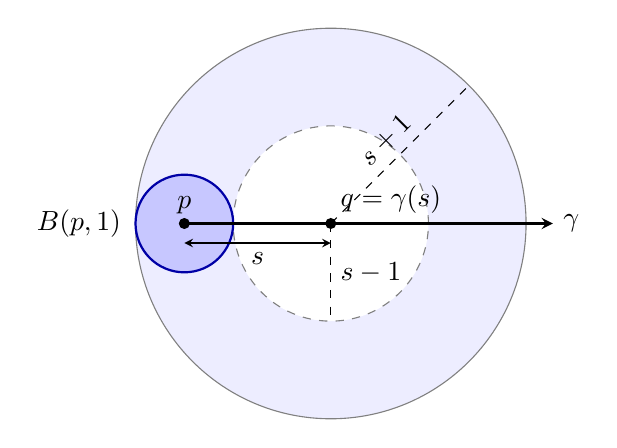
\begin{tikzpicture}[x=.62cm,y=.62cm,>=stealth]
	\fill[blue!7] (0,0) circle (4);
	\fill[white] (0,0) circle (2);
	\draw[gray] (0,0) circle (4);
	\draw[gray,dashed] (0,0) circle (2);
	\filldraw[fill=blue!22,draw=blue!65!black,thick] (-3,0) circle (1);
	\draw[thick,->] (-3,0)--(4.55,0) node[right] {\(\gamma\)};
	\draw[dashed] (0,0)--(2.828,2.828) node[midway,above,sloped] {\(s+1\)};
	\draw[dashed] (0,0)--(0,-2) node[midway,right] {\(s-1\)};
	\draw[<->] (-3,-.4)--(0,-.4) node[midway,below] {\(s\)};
	\fill (-3,0) circle (2pt) node[above] {\(p\)};
	\fill (0,0) circle (2pt) node[above right] {\(q=\gamma(s)\)};
	\node[left] at (-4.1,0) {\(B(p,1)\)};
\end{tikzpicture}

	\caption{把中心移到射线远点 \(q=\gamma(s)\) 后，固定小球落入半径 \(s-1\) 与 \(s+1\) 之间的球壳。图中的圆示意测地球，包含关系由三角不等式保证。}
	\label{g3:fig:ray-annulus}
\end{figure}

\cref{g3:fig:ray-annulus}显示了换球心的作用：小球本身未变，但容纳它的球壳厚度固定为2，相对半径却越来越小。球壳比较因此迫使大球体积随半径增长。下界的常数保留了 \(V_p(1)\)：非负 Ricci 曲率并不为单位球提供一个只依赖维数的正体积下界。例如，将平坦环面的周长缩小，\(\mathbb R\times T^{n-1}\) 的单位球体积也会变小。

\subsection{覆盖空间中的体积计数}
\label{g3:subsec:0803:02}

设 \(\pi:\widetilde M\to M\) 为万有覆盖，赋予 \(\widetilde M\) 拉回度量 \(\widetilde g=\pi^*g\)。由\cref{g3:prop:riemannian-cover-complete}，基流形完备时，覆盖空间也完备。覆盖变换群 \(\Gamma\) 的每个元素都是等距映射，因为 \(\pi\circ h=\pi\) 蕴含 \(h^*\widetilde g=\widetilde g\)。它在每条纤维上自由且传递，因而给定 \(\widetilde p\in\pi^{-1}(p)\) 后，群元素与轨道点 \(h\widetilde p\) 一一对应。

\begin{proposition}\label{g3:prop:covering-orbit-count}
	设 \((M^n,g)\) 为连通、完备、光滑无边界黎曼流形，\(\pi:(\widetilde M,\widetilde g)\to(M,g)\) 为带拉回度量的万有覆盖，\(\Gamma\) 为覆盖变换群。固定 \(\widetilde p\in\widetilde M\)。存在 \(\varepsilon>0\)，使开球族
	\[
		\{B_{\widetilde g}(h\widetilde p,\varepsilon):h\in\Gamma\}
	\]
	两两不交。记 \(v_\varepsilon=\operatorname{Vol}_{\widetilde g}B(\widetilde p,\varepsilon)\)，以及
	\[
		N_{\widetilde p}(R)
		=\#\{h\in\Gamma:
		d_{\widetilde g}(\widetilde p,h\widetilde p)\le R\}.
	\]
	则 \(0<v_\varepsilon<\infty\)，每个 \(N_{\widetilde p}(R)\) 有限，并且
	\begin{equation}\label{g3:eq:covering-volume-packing}
		N_{\widetilde p}(R)v_\varepsilon
		\le\operatorname{Vol}_{\widetilde g}B(\widetilde p,R+\varepsilon)
		\qquad(R\ge0).
	\end{equation}
	若进一步有 \(n\ge2\) 且 \(\operatorname{Ric}_g\ge0\)，则
	\begin{equation}\label{g3:eq:covering-polynomial-orbit}
		N_{\widetilde p}(R)
		\le\frac{\omega_n}{v_\varepsilon}(R+\varepsilon)^n.
	\end{equation}
\end{proposition}
\begin{proof}
	取 \(p=\pi(\widetilde p)\) 的连通均匀覆盖邻域 \(U\)，并令 \(W\) 是 \(\pi^{-1}(U)\) 中含 \(\widetilde p\) 的那一层。对任意 \(h\in\Gamma\)，集合 \(hW\) 也是一层。若 \(hW=W\)，则 \(\pi|_W\) 的单射性与 \(\pi\circ h=\pi\) 给出 \(h|_W=\mathrm{id}\)。覆盖变换由一点的像唯一确定，所以此时 \(h=\mathrm{id}\)。因此不同覆盖变换给出的层 \(hW\) 两两不交。

	距离拓扑等于流形拓扑，可以选 \(\varepsilon>0\)，使 \(B(\widetilde p,\varepsilon)\subset W\)。等距性给出
	\[
		B(h\widetilde p,\varepsilon)
		=hB(\widetilde p,\varepsilon)\subset hW,
	\]
	故这些小球两两不交，体积都等于 \(v_\varepsilon\)。光滑正体积密度保证 \(v_\varepsilon>0\)；覆盖空间完备，其闭有界球紧，故 \(v_\varepsilon<\infty\)。

	当 \(d(\widetilde p,h\widetilde p)\le R\) 时，三角不等式给出
	\[
		B(h\widetilde p,\varepsilon)
		\subset B(\widetilde p,R+\varepsilon).
	\]
	对满足此条件的任意有限个群元素，把相应小球的体积相加，所得结果不超过右侧大球的体积。后者有限而 \(v_\varepsilon>0\)，所以这样的群元素总数必然有限，并得到\eqref{g3:eq:covering-volume-packing}。

	最后，局部等距保持 Ricci 曲率及度量不等式，所以 \(\operatorname{Ric}_{\widetilde g}\ge0\)。在完备的覆盖空间上应用\cref{g3:thm:bishop-gromov}，得
	\[
		\operatorname{Vol}_{\widetilde g}B(\widetilde p,R+\varepsilon)
		\le\omega_n(R+\varepsilon)^n.
	\]
	代回即得\eqref{g3:eq:covering-polynomial-orbit}。
\end{proof}

这里计数的是覆盖空间中的轨道，右端也必须使用覆盖空间的体积。基流形中的大球会把不同提升识别为同一点，其体积通常不能替代\eqref{g3:eq:covering-volume-packing}的右端。平坦乘积的例子将显示，这一区别会改变增长的次数。

\subsection{有限生成子群的增长约束}
\label{g3:subsec:0803:03}

体积估计控制的是几何位移。为了把它用于抽象群，需选定有限个生成元，并记录至多使用多少个生成元能够到达一个元素。

\begin{definition}\label{g3:def:word-growth}
	设 \(G\) 为群，\(S\subset G\) 为有限对称生成集，即 \(S^{-1}=S\) 且 \(S\) 生成 \(G\)。元素 \(h\in G\) 的\term[zichang]{字长}[word length]定义为
	\[
		|h|_S=\min\{m\ge0:h=s_1\cdots s_m,\ s_i\in S\},
	\]
	其中空乘积表示单位元。记
	\[
		\mathcal B_S(m)=\{h\in G:|h|_S\le m\},
		\qquad \beta_S(m)=\#\mathcal B_S(m).
	\]
	若存在 \(C>0\)，使所有整数 \(m\ge0\) 都满足
	\(\beta_S(m)\le C(m+1)^d\)，则称 \(G\) 具有次数至多为 \(d\) 的\term[duoxiangshizengzhang]{多项式增长}[polynomial growth]。
\end{definition}

这一性质不依赖有限生成集的选择。事实上，若 \(T\) 是另一有限对称生成集，取
\[
	A=\max\bigl(\{1\}\cup\{|s|_T:s\in S\}\bigr),
\]
把每个 \(S\) 中的字母换成至多 \(A\) 个 \(T\) 中的字母，便得到
\(\mathcal B_S(m)\subset\mathcal B_T(Am)\)。交换 \(S,T\) 得到反向的线性尺度比较。因此，多项式上界的次数可以保持，常数则随生成集变化。

\begin{theorem}\label{g3:thm:fundamental-subgroup-growth}
	设 \((M^n,g)\) 为连通、完备、光滑无边界黎曼流形，\(n\ge2\)，且 \(\operatorname{Ric}\ge0\)。则 \(\pi_1(M,p)\) 的每个有限生成子群 \(G\)，相对于任意有限对称生成集 \(S\)，都满足
	\[
		\beta_S(m)\le C_S(m+1)^n
		\qquad(m=0,1,2,\ldots),
	\]
	其中 \(C_S\) 可以依赖流形、基点、子群和生成集。
\end{theorem}
\begin{proof}
	利用万有覆盖的覆盖变换群与基本群的同构，将 \(G\) 看成覆盖变换群 \(\Gamma\) 的子群。选定 \(\widetilde p\in\pi^{-1}(p)\)。若 \(G\) 为平凡群，结论由 \(\beta_S(m)=1\) 得到；以下设 \(G\) 非平凡，并在生成集中删去单位元。令
	\[
		L=\max_{s\in S}d_{\widetilde g}(\widetilde p,s\widetilde p)>0.
	\]
	覆盖变换等距，因此任意 \(g,h\in\Gamma\) 满足
	\[
		d(\widetilde p,gh\widetilde p)
		\le d(\widetilde p,g\widetilde p)
		+d(g\widetilde p,gh\widetilde p)
		=d(\widetilde p,g\widetilde p)
		+d(\widetilde p,h\widetilde p).
	\]
	反复应用可知，若 \(|h|_S\le m\)，则
	\(d(\widetilde p,h\widetilde p)\le mL\)。不同群元素作用于 \(\widetilde p\) 得到不同点，所以
	\[
		\beta_S(m)\le N_{\widetilde p}(mL).
	\]
	应用\cref{g3:prop:covering-orbit-count}，得到
	\[
		\beta_S(m)
		\le\frac{\omega_n}{v_\varepsilon}(mL+\varepsilon)^n
		\le\frac{\omega_n(L+\varepsilon)^n}{v_\varepsilon}(m+1)^n.
	\]
	取最后一个系数为 \(C_S\) 即可。
\end{proof}

定理的量词逐个作用于有限生成子群。证明中，有限生成性恰好用于取得生成元位移的有限上界 \(L\)；所得估计本身没有给出整个基本群的一组有限生成元。另一个直接用途是排除增长过快的子群。例如，自由群 \(F_2=\langle a,b\rangle\) 相对于 \(\{a,a^{-1},b,b^{-1}\}\)，长度恰为 \(m\ge1\) 的约化字有 \(4\cdot3^{m-1}\) 个：第一个字母有四种选择，此后每次排除前一字母的逆元，尚有三种选择。因此 \(F_2\) 不可能作为上述基本群的子群。

\subsection{Euclid、双曲及乘积模型}
\label{g3:subsec:0803:04}

模型计算同时检验小尺度和大尺度。光滑 \(n\) 维度量的小球都有 \(n\) 维 Euclid 主项；大球则会反映曲率累积以及紧方向被填满之后的变化。

\begin{example}\label{g3:exm:euclidean-hyperbolic-volume-growth}
	在 Euclid 空间 \(\mathbb R^n\) 中，
	\[
		V_p(R)=\omega_nR^n
	\]
	对所有 \(R>0\) 成立。对曲率为 \(-a^2\) 的双曲模型，取 \(a>0\)、\(n\ge2\)，其全局极坐标度量为
	\[
		g=\mathrm dr^2+
		\left(\frac{\sinh(ar)}a\right)^2g_{S^{n-1}}.
	\]
	这里全局坐标可由双曲面
	\[
		-x_0^2+|x|^2=-a^{-2},\qquad x_0>0
	\]
	上的参数式
	\[
		x_0=a^{-1}\cosh(ar),\qquad
		x=a^{-1}\sinh(ar)u,\qquad u\in S^{n-1},
	\]
	直接得到：将其微分代入 \(-\mathrm dx_0^2+|\mathrm dx|^2\)，径向项为 \(\mathrm dr^2\)，角向项为 \((\sinh(ar)/a)^2g_{S^{n-1}}\)，交叉项为零。每条从中心到半径 \(r\) 的曲线长度至少为 \(r\)，因为离开中心后其速度长度不小于径向速度的绝对值；径向曲线达到此下界。故坐标半径就是中心距离，球体积为
	\begin{equation}\label{g3:eq:hyperbolic-volume-growth}
		V_{-a^2,n}(R)
		=\frac{\sigma_{n-1}}{a^{n-1}}
		\int_0^R\sinh(at)^{n-1}\,\mathrm dt.
	\end{equation}
	当 \(R\downarrow0\) 时，\(\sinh(at)/a=t+O(t^3)\)，所以
	\[
		V_{-a^2,n}(R)=\omega_nR^n\bigl(1+O(R^2)\bigr).
	\]
	当 \(R\to\infty\) 时，
	\[
		\sinh(aR)^{n-1}
		\sim 2^{-(n-1)}e^{(n-1)aR}.
	\]
	将积分与 \(e^{(n-1)aR}\) 的比求极限，或对这个渐近式积分，得到
	\begin{equation}\label{g3:eq:hyperbolic-volume-asymptotic}
		V_{-a^2,n}(R)
		\sim
		\frac{\sigma_{n-1}}{2^{n-1}(n-1)a^n}
		e^{(n-1)aR}.
	\end{equation}
	例如 \(n=2\) 时可直接积分：
	\[
		V_{-a^2,2}(R)=\frac{2\pi}{a^2}\bigl(\cosh(aR)-1\bigr).
	\]
	这里的指数增长说明，非负 Ricci 假设对多项式体积上界具有实质作用。
\end{example}

\begin{example}\label{g3:exm:flat-product-volume-growth}
	设 \(a,b\ge1\) 为整数，\(T^b=\mathbb R^b/\Lambda\) 为平坦环面，赋予
	\[
		M=\mathbb R^a\times T^b
	\]
	乘积度量。其总维数为 \(n=a+b\)，曲率恒为零。记环面直径为 \(D>0\)、体积为 \(v_T>0\)，固定中心 \((0,y_0)\)。

	先核对距离。任意从 \((0,y_0)\) 到 \((x,y)\) 的分片光滑曲线 \((\alpha,\beta)\) 都满足
	\[
		\int\sqrt{|\dot\alpha|^2+|\dot\beta|^2}
		\ge
		\sqrt{\left(\int|\dot\alpha|\right)^2+
		\left(\int|\dot\beta|\right)^2}
		\ge\sqrt{|x|^2+d_T(y_0,y)^2}.
	\]
	第一个不等式是对向量值函数
	\((|\dot\alpha|,|\dot\beta|)\) 的积分三角不等式。反过来，分别取两个因子中的最短线，并将它们参数化在 \([0,1]\) 上，使速度长度恒为各自端点距离，便达到下界。因此
	\[
		d_M((0,y_0),(x,y))^2=|x|^2+d_T(y_0,y)^2.
	\]
	两个因子均完备，距离公式又说明乘积中的 Cauchy 序列逐分量收敛，所以 \(M\) 完备。

	用乘积体积密度逐纤维积分，可得对所有 \(R>0\) 都成立的精确公式
	\begin{equation}\label{g3:eq:flat-product-volume-formula}
		V_{(0,y_0)}(R)
		=\omega_a\int_{T^b}
		\bigl(R^2-d_T(y_0,y)^2\bigr)_+^{a/2}\,\mu_T(y),
	\end{equation}
	其中 \(s_+=\max\{s,0\}\)。因为 \(0\le d_T(y_0,y)\le D\)，当 \(R>D\) 时，
	\begin{equation}\label{g3:eq:flat-product-volume-bounds}
		\omega_av_T(R^2-D^2)^{a/2}
		\le V_{(0,y_0)}(R)
		\le\omega_av_TR^a.
	\end{equation}
	特别地，对 \(R\ge2D\)，有
	\[
		\left(\frac34\right)^{a/2}\omega_av_TR^a
		\le V_{(0,y_0)}(R)
		\le\omega_av_TR^a,
	\]
	而令 \(R\to\infty\) 得到
	\[
		V_{(0,y_0)}(R)\sim\omega_av_TR^a.
	\]

	小尺度却仍是 \(n=a+b\) 维的。设
	\(\rho=\frac12\min_{\lambda\in\Lambda\setminus\{0\}}|\lambda|>0\)。
	当 \(0<R<\rho\) 时，覆盖映射
	\(\mathbb R^{a+b}\to\mathbb R^a\times T^b\)
	在 Euclid 半径 \(R\) 的球上限制为到上述球的微分同胚，并保持黎曼度量：任意 \(y\) 的最短代表可由使 \(|\widetilde y+\lambda|\) 最小的格点给出，距离公式保证满射；两个球内点若相差非零格向量，其距离小于 \(2R<2\rho\)，又与格向量长度下界矛盾。因此
	\[
		V_{(0,y_0)}(R)=\omega_{a+b}R^{a+b}
		\qquad(0<R<\rho).
	\]
	公式\eqref{g3:eq:flat-product-volume-formula}描述了从小尺度到大尺度的整个过渡。当 \(a=1\) 时，大球体积恰为线性量级，说明\cref{g3:thm:noncompact-volume-growth}的线性下界在一般情形下不能提高到更大的幂次。
\end{example}

上述乘积的万有覆盖是 \(\mathbb R^{a+b}\)，覆盖变换沿环面因子的格点作平移。因此，基流形的大球按 \(R^a\) 增长，覆盖空间的大球却按 \(R^{a+b}\) 增长。覆盖体积计数使用后一个增长率，正是因为它需要把所有不同提升的小球分别容纳进去。
% 纲要条目排为编号小节标题，并进入目录与书签；说明段仍保留于纲要注释中。

% !TeX root = ../../Book3.tex
% 纲要标题：### 8.4 曲率比较的适用范围
% 纲要位置：几何学计划纲要.md，第 2418 行。
% 正文状态：初稿；尚未正式审核。

% 纲要内容开始
% 
% * 非负 Ricci 与非负截面曲率的区别
% * 塌缩时体积信息的变化
% * Busemann 函数与分裂定理
% 
% ---
% 
% 纲要内容结束

\section{曲率比较的适用范围}
\label{g3:sec:0804}

本章的比较把曲率信息逐步变成长度、体积与群的计数。取迹和积分使这些结论适用范围很广，也会丢失某些方向与尺度的信息。本节用具体模型辨别这些损失，再考察从距离比较走向整体乘积分解还需要哪些工具。

\subsection{非负 Ricci 与非负截面曲率的区别}
\label{g3:subsec:0804:01}

若 \(T,e_1,\ldots,e_{n-1}\) 是一点处的正交单位基，则
\[
	\operatorname{Ric}(T,T)=\sum_{i=1}^{n-1}K(T\wedge e_i).
\]
因此 \(K\ge k\) 推出 \(\operatorname{Ric}\ge(n-1)kg\)。二维只有一个截面，\(\operatorname{Ric}=Kg\)，这两个条件等价；从三维起，一个方向的负截面曲率可以被其他方向的正曲率补偿。

例如\cref{g3:exm:ricci-positive-sectional-negative}给出的三维代数曲率张量满足
\[
	K(e_1\wedge e_2)=-1,\qquad
	K(e_1\wedge e_3)=K(e_2\wedge e_3)=2,
	\qquad \operatorname{Ric}=\operatorname{diag}(1,1,4).
\]
\Cref{g3:prop:curvature-local-realization}把它实现为一点附近的光滑度量，严格正的 Ricci 与指定的负截面在足够小的邻域中同时保留。这说明即使在局部，正 Ricci 也不能替代逐截面的正性；该构造本身没有给出全局的 Ricci 下界。第七章的迹比较正好体现这个区别：它控制径向形算子的迹，而不能分别控制其全部特征值。只有达到模型等号时，平方和估计的等号才进一步迫使各个特征值相等。

另一种容易混淆的条件是“处处严格为正”和“有统一的正常数下界”。后者是本章直径定理真正使用的条件。

\begin{example}\label{g3:exm:positive-paraboloid}
	考虑 Euclid 空间中的抛物面
	\[
		P=\{(x,y,z)\in\mathbb R^3:z=x^2+y^2\},
	\]
	赋予诱导度量。用水平极坐标 \((\rho,\theta)\) 表示，得到
	\[
		g=(1+4\rho^2)\,\mathrm d\rho^2+\rho^2\,\mathrm d\theta^2.
	\]
	在全局图坐标 \((x,y)\) 中，\(g=\mathrm dx^2+\mathrm dy^2+4(x\,\mathrm dx+y\,\mathrm dy)^2\ge g_{\mathrm E}\)。所以任一 \(g\)-Cauchy 序列在 Euclid 坐标中收敛；在极限点的紧坐标邻域中，\(g\le Cg_{\mathrm E}\)，它也按 \(g\) 收敛。这证明 \(P\) 完备。全局图坐标又表明它非紧。

	令 \(s(\rho)=\int_0^\rho\sqrt{1+4u^2}\,\mathrm du\)，把度量写成 \(\mathrm ds^2+f(s)^2\mathrm d\theta^2\)，其中 \(f(s)=\rho\)。于是
	\[
		f'(s)=\frac1{\sqrt{1+4\rho^2}},\qquad
		f''(s)=-\frac{4\rho}{(1+4\rho^2)^2}.
	\]
	由\cref{g3:prop:warped-product-curvature}，在 \(\rho>0\) 处
	\[
		K=-\frac{f''}{f}=\frac4{(1+4\rho^2)^2}>0.
	\]
	在顶点处由光滑性取极限仍得 \(K=4\)。因此 \(\operatorname{Ric}=Kg\) 处处正定，但 \(K\to0\) 于无穷远，不能选取本章直径定理所需的统一 \(k>0\)。
\end{example}

这个例子也把两个尺度联系起来：每一点附近都有正曲率的局部几何，远处越来越小的曲率却容许测地线无限延伸。章末将直接计算其球面积，得到介于线性与二次之间的增长。

\subsection{塌缩时体积信息的变化}
\label{g3:subsec:0804:02}

体积比较给出上界以及不同半径之间的比值控制。它是否同时给出某个固定半径球的一致正体积下界？以下平坦例子说明，还必须指定一个不退化的体积尺度。

\begin{example}\label{g3:exm:collapsing-flat-tori}
	设 \(n\ge2\)、\(0<\varepsilon\le1\)，取平坦乘积
	\[
		T_\varepsilon=(\mathbb R/\mathbb Z)^{n-1}
		\times(\mathbb R/\varepsilon\mathbb Z).
	\]
	它的曲率恒为零，基本区域的体积为 \(\varepsilon\)。乘积距离由各个圆周的最短弧长平方求和得到，故
	\[
		\operatorname{diam}T_\varepsilon
		=\frac12\sqrt{n-1+\varepsilon^2},\qquad
		\operatorname{inj}(T_\varepsilon)=\frac\varepsilon2.
	\]
	最后一式也可从格商看出：长度最短的非零格向量为 \(\varepsilon\)，指数映射在半径小于其一半时单射，在一半处遇到相反的最短弧。

	固定一点 \(p\)，仍以 \(\omega_j\) 表示 Euclid 单位 \(j\) 维球体积。若 \(r<\varepsilon/2\)，则 \(B(p,r)\) 是 Euclid 球，体积恰为 \(\omega_n r^n\)。若 \(\varepsilon/2<r<1/2\)，短圆周上的所有点距离基点都不超过 \(\varepsilon/2\)，于是
	\begin{equation}\label{g3:eq:collapsed-ball-estimate}
		\varepsilon\omega_{n-1}(r^2-\varepsilon^2/4)^{(n-1)/2}
		\le\operatorname{Vol}_g B(p,r)
		\le\varepsilon\omega_{n-1}r^{n-1}.
	\end{equation}
	确切地说，球内含半径 \(\sqrt{r^2-\varepsilon^2/4}\) 的底空间球与整条短圆周的乘积，并包含于半径 \(r\) 的底空间球与短圆周的乘积；在 \(r<1/2\) 时这些底空间球均为 Euclid 球。这就证明了两侧体积估计。

	固定 \(0<r<1/2\) 并令 \(\varepsilon\downarrow0\)，有
	\[
		\operatorname{Vol}_g B(p,r)\longrightarrow0,
		\qquad
		\frac{\operatorname{Vol}_g B(p,r)}\varepsilon
		\longrightarrow\omega_{n-1}r^{n-1}.
	\]
	投影 \(\pi:T_\varepsilon\to(\mathbb R/\mathbb Z)^{n-1}\) 还满足
	\[
		d(\pi x,\pi y)\le d(x,y)
		\le\sqrt{d(\pi x,\pi y)^2+\varepsilon^2/4}
		\le d(\pi x,\pi y)+\varepsilon/2.
	\]
	因此短圆周方向在固定尺度的距离测量中逐渐消失；体积趋零和距离趋近低一维空间发生在同一模型中。
\end{example}

这种有些方向的长度尺度趋零、相应体积退化的现象称为\term[tasuo]{塌缩}[collapse]。在上例中，先固定 \(\varepsilon\) 再令 \(r\downarrow0\)，总能看到 \(n\) 维 Euclid 体积；先固定 \(r\) 再令 \(\varepsilon\downarrow0\)，却会失去一个方向。小球的局部维数与一族度量在固定尺度下的退化因而是不同问题。

给定尺度上的一致正体积下界通常称为该尺度的\term[fei tansuo]{非塌缩}[noncollapse]条件。体积比较能够把已有的这种下界传到邻近中心及更小半径。

\begin{proposition}\label{g3:prop:noncollapse-propagation}
	记 \(V_p(r)=\operatorname{Vol}_g B(p,r)\)，\(\sigma_{n-1}\) 为 Euclid 单位球面的面积，\(V_{k,n}(r)=\sigma_{n-1}\int_0^r s_k(t)^{n-1}\,\mathrm dt\) 为常曲率模型球体积。
	取 \(k\in\mathbb R\)。记 \(s_k\) 为 \(s_k''+ks_k=0\)、\(s_k(0)=0\)、\(s_k'(0)=1\) 的解，\(b_k=\pi/\sqrt k\) 当 \(k>0\)，否则 \(b_k=\infty\)。
	设 \((M^n,g)\) 连通、完备、光滑且无边界，\(n\ge2\)，\(\operatorname{Ric}\ge(n-1)kg\)。设 \(p,q\in M\)、\(d(p,q)\le D\)，且 \(r_0>0\)、\(\operatorname{Vol}_g B(p,r_0)\ge v_0>0\)。若 \(0<r\le D+r_0<b_k\)，则
	\[
		\operatorname{Vol}_g B(q,r)
		\ge\frac{V_{k,n}(r)}{V_{k,n}(D+r_0)}v_0.
	\]
\end{proposition}
\begin{proof}
	三角不等式给出 \(B(p,r_0)\subset B(q,D+r_0)\)。把\cref{g3:thm:bishop-gromov}用于中心 \(q\) 以及半径 \(r,D+r_0\)，得
	\[
		\frac{\operatorname{Vol}_g B(q,r)}{V_{k,n}(r)}
		\ge\frac{\operatorname{Vol}_g B(q,D+r_0)}{V_{k,n}(D+r_0)}
		\ge\frac{v_0}{V_{k,n}(D+r_0)}.
	\]
\end{proof}

特别地，当 \(\operatorname{Ric}\ge0\) 时，下界变成 \(v_0(r/(D+r_0))^n\)，且没有有限的模型半径限制。这里体积的绝对尺度来自假设中的 \(v_0\)；曲率比较负责传播它。平坦环面族中这个初始体积本身趋零，所以与该命题完全相容。

\subsection{Busemann 函数与分裂定理}
\label{g3:subsec:0804:03}

在 Euclid 空间中，一条定向直线给出一个线性坐标；与它垂直的超平面组成一个乘积分解。在一般完备流形中，可以先把测地射线上的点推向无穷远，再从距离中减去趋于无穷的常数，尝试得到相应坐标。

\begin{definition}\label{g3:def:busemann-function}
	设 \((M,g)\) 是连通、完备、光滑无边界黎曼流形，\(\gamma:[0,\infty)\to M\) 为单位速测地射线，即 \(d(\gamma(s),\gamma(t))=|s-t|\)。函数
	\begin{equation}\label{g3:eq:busemann-sign}
		b_\gamma(x)=\lim_{t\to\infty}\bigl(t-d(x,\gamma(t))\bigr)
	\end{equation}
	称为 \(\gamma\) 的\term[Busemann hanshu]{Busemann 函数}[Busemann function]。\footnote{Herbert Busemann（1905--1994），德国出生的美国数学家，研究度量几何、凸性与测地线。}本书采用沿射线增加的符号，因而下面将有 \(b_\gamma(\gamma(s))=s\)。
\end{definition}

\symidx{\(b_\gamma\)：沿射线增加的 Busemann 函数}
定义中的极限并不要求曲率条件，其存在性来自三角不等式。完备非紧流形上已有\cref{g3:lem:complete-noncompact-ray}保证这样的射线存在。

\begin{proposition}\label{g3:prop:busemann-basic}
	设 \((M,g)\) 连通、完备、光滑且无边界，\(\gamma:[0,\infty)\to M\) 为单位速测地射线。则式\eqref{g3:eq:busemann-sign}的极限处处存在，且在每个紧集上一致收敛。函数 \(b_\gamma\) 为1-Lipschitz，满足
	\[
		|b_\gamma(x)|\le d(x,\gamma(0)),\qquad
		b_\gamma(\gamma(s))=s\quad(s\ge0).
	\]
\end{proposition}
\begin{proof}
	记 \(b_t(x)=t-d(x,\gamma(t))\)。对 \(t\ge s\)，由射线的最短性及三角不等式，
	\[
		d(x,\gamma(t))\le d(x,\gamma(s))+t-s,
		\qquad b_t(x)\ge b_s(x).
	\]
	又由三角不等式的两种写法，\(-d(x,\gamma(0))\le b_t(x)\le d(x,\gamma(0))\)。所以 \(b_t(x)\) 单调有界，极限存在。每个 \(b_t\) 都为1-Lipschitz，取极限保留这一性质及上述界。在射线上，对 \(t\ge s\) 直接计算 \(b_t(\gamma(s))=t-(t-s)=s\)。

	最后设 \(K\subset M\) 紧。任给 \(\eta>0\)，取有限个半径 \(\eta\) 的球覆盖 \(K\)，球心取在 \(K\) 中。在这有限个球心上，当 \(t\) 足够大时均有 \(|b_t-b_\gamma|<\eta\)。对任一 \(x\in K\)，选取相距小于 \(\eta\) 的球心；使用 \(b_t,b_\gamma\) 的1-Lipschitz 性，得到 \(|b_t(x)-b_\gamma(x)|<3\eta\)。这证明紧集上的一致收敛。
\end{proof}

在 \(\mathbb R^n\) 中取 \(\gamma(t)=tv\)、\(|v|=1\)。有理化给出
\[
	 t-|x-tv|
	=\frac{2t\langle x,v\rangle-|x|^2}{t+|x-tv|}
	\longrightarrow\langle x,v\rangle.
\]
因此这一极限确实恢复沿 \(v\) 的线性坐标。一般流形上的 \(b_\gamma\) 首先只有 Lipschitz 正则性；距离函数的割迹也不能在取极限时直接忽略。第七章的分布比较正好适用于这一过程。

\begin{proposition}\label{g3:prop:busemann-weak-laplacian}
	设 \((M^n,g)\) 连通、完备、光滑且无边界，\(n\ge2\)，\(\operatorname{Ric}\ge0\)，\(\gamma\) 为单位速测地射线。以 \(\Delta=-\operatorname{div}\nabla\) 记本书的 Laplace 算子，则
	\[
		\Delta b_\gamma\le0
	\]
	在分布意义下成立，即对每个非负 \(\phi\in C_c^\infty(M)\)，\(\int_M b_\gamma\Delta\phi\,\mu_g\le0\)。
\end{proposition}
\begin{proof}
	令 \(K=\operatorname{supp}\phi\)，取 \(C\) 使 \(d(x,\gamma(0))\le C\) 对 \(x\in K\) 成立。若 \(t>C\)，则 \(r_t(x)=d(x,\gamma(t))\ge t-C>0\) 于 \(K\)。由\cref{g3:thm:distributional-laplacian-comparison}在 \(k=0\) 时的结论，\(\Delta r_t\ge-(n-1)/r_t\)。又因紧支测试函数满足 \(\int_M\Delta\phi\,\mu_g=0\)，有
	\[
		\int_M b_t\Delta\phi\,\mu_g
		=-\int_M r_t\Delta\phi\,\mu_g
		\le\int_M\frac{n-1}{r_t}\phi\,\mu_g
		\le\frac{n-1}{t-C}\int_M\phi\,\mu_g.
	\]
	在 \(K\) 上 \(b_t\) 一致趋于 \(b_\gamma\)，令 \(t\to\infty\)，右端趋于零，即得所需分布不等式。
\end{proof}

设现在有一条\term[cedi zhixian]{测地直线}[geodesic line] \(\gamma:\mathbb R\to M\)，即单位速测地线且任意有限段都最短，等价地 \(d(\gamma(s),\gamma(t))=|s-t|\)。对它的两个方向分别构造
\[
	 b_+(x)=\lim_{t\to\infty}\bigl(t-d(x,\gamma(t))\bigr),\qquad
	 b_-(x)=\lim_{t\to\infty}\bigl(t-d(x,\gamma(-t))\bigr).
\]
三角不等式给出 \(d(x,\gamma(t))+d(x,\gamma(-t))\ge2t\)，所以
\begin{equation}\label{g3:eq:two-busemann-functions}
	 b_++b_-\le0,\qquad
	 b_+(\gamma(s))+b_-(\gamma(s))=s-s=0.
\end{equation}
若 \(\operatorname{Ric}\ge0\)，两者又满足 \(\Delta b_\pm\le0\)。于是 \(b_++b_-\) 是一个在直线上达到全局最大值的弱次调和函数；这里“次调和”对应 \(\operatorname{div}\nabla\ge0\)，也就是本书的 \(\Delta\le0\)。

要把这一事实变成乘积分解，还需三步分析。首先，用适用于上述弱不等式的强最大值原理推出 \(b_++b_-=0\)，从而两者弱调和；其次，用椭圆正则性取得光滑性，并借从任意点出发的渐近射线证明 \(|\nabla b_+|=1\)；最后用 Bochner 公式推出 \(\operatorname{Hess}b_+=0\)。这时 \(\nabla b_+\) 才成为平行单位场，其流把等值面与实直线组成整体等距乘积。

这些步骤及所需的弱最大值、正则性工具将在\secref{g3:sec:1505}汇合，证明如下结论：若 \((M^n,g)\) 连通、完备、光滑、无边界且 \(\operatorname{Ric}\ge0\)，并含有一条测地直线，则 \(M\) 等距于 \(\mathbb R\times N\)，其中 \(N\) 是完备的 \((n-1)\) 维黎曼流形。这里要求的是双向都保持最短的直线；单有从一点出发的射线，只保证 Busemann 函数存在，尚不能使式\eqref{g3:eq:two-busemann-functions}的两侧构造成立。
% 纲要条目排为编号小节标题，并进入目录与书签；说明段仍保留于纲要注释中。


\begin{chaptersummary}
	固定端点的正弦试探场把 Ricci 的统一正下界变成最短线长度的上界。完备性提供最短线并把有界性提升为紧性；把相同论证用于拉回度量下的万有覆盖，再以紧离散纤维计数，就得到基本群有限性。

	\ProseParagraphBreak

	径向密度除以模型密度后不增，在割时的向下跳跃保留了这一方向。沿球面与半径积分，便得到球体积比及球壳的相对比较；最大体积的等号同时排除球内割点和径向伸缩中的亏损，因而恢复模型球的度量。将球心移向射线远处给出非紧流形的线性体积下界，在覆盖中放入两两不交的小球则把体积上界变成轨道与群的增长上界。

	\ProseParagraphBreak

	Ricci 条件控制方向和，塌缩模型说明它也不能单独固定一个正体积尺度。射线的 Busemann 函数把距离比较传到无穷远，但其最初的正则性只有 Lipschitz；由弱 Laplace 不等式取得光滑平行梯度，需要后续的最大值原理、椭圆正则性与 Bochner 公式。下一章将回到截面曲率，研究全局指数映射、空间形式与测地三角比较；度量收敛与塌缩的系统语言在第十章建立。
\end{chaptersummary}

\BookExercises

\begin{exercise}\label{g3:ex:myers-unbounded-finite-group-order}
	在单位球面
	\[
		S^3=\{(z_1,z_2)\in\mathbb C^2:|z_1|^2+|z_2|^2=1\}
	\]
	上取圆度量。对整数 \(m\ge2\)，令 \(\zeta=e^{2\pi\mathrm{i}/m}\)，以
	\[
		A(z_1,z_2)=(\zeta z_1,\zeta z_2)
	\]
	生成循环群 \(\Gamma_m\)。证明商 \(M_m=S^3/\Gamma_m\) 是紧连通无边界光滑三维流形，具有截面曲率恒为 \(1\) 的商度量，并且
	\[
		\operatorname{Ric}_{M_m}=2g_m,\qquad
		\operatorname{diam}(M_m)\le\pi,\qquad
		\pi_1(M_m)\cong\mathbb Z/m\mathbb Z.
	\]
	据此说明，固定维数、正 Ricci 下界和直径上界，仍不能由 Bonnet--Myers 定理得到基本群阶的统一上界。
\end{exercise}
\begin{solution}
	\(A\) 是 \(\mathbb R^4\) 上的正交变换，因此保持球面及圆度量。若 \(A^jz=z\)，至少有一个 \(z_i\ne0\)，故 \(\zeta^j=1\)，即 \(m\mid j\)。所以群作用自由，且每条轨道恰有 \(m\) 个点。

	在每个 \(z\in S^3\) 处，选小球 \(U\)，使 \(U,A(U),\ldots,A^{m-1}(U)\) 两两不交；有限轨道中不同点的正距离保证可以这样取。商投影限制到 \(U\) 为同胚，利用这些限制把球面坐标送到商上，过渡映射是原坐标变换与某个 \(A^j\) 的复合，因而光滑。不同有限轨道可取互不相交的饱和邻域，故商 Hausdorff；商映射开，球面的可数基之像给出商的可数基。因此商确为光滑三维无边界流形，投影为 \(m\) 叶光滑覆盖。商还是紧连通空间，因为它是紧连通球面的连续像。

	各 \(A^j\) 为等距变换，故局部搬运的度量在覆盖片之间一致，给出使投影局部等距的商度量。局部等距保持曲率，所以 \(K_{M_m}=1\)、\(\operatorname{Ric}_{M_m}=2g_m\)。紧性给出完备性，\cref{g3:thm:bonnet-myers}在 \(n=3,k=1\) 时得到直径界 \(\pi\)。

	第一卷第5章第2节“高维球面的单连通性”命题给出 \(S^3\) 单连通，故此覆盖就是万有覆盖。其覆盖变换群恰为 \(\Gamma_m\)：已给变换在一个纤维上传递，而任意覆盖变换由一点的像唯一确定，不可能还有其他变换。第一卷第5章第4节的万有覆盖变换群结论于是给出 \(\pi_1(M_m)\cong\Gamma_m\cong\mathbb Z/m\mathbb Z\)。当 \(m\to\infty\) 时，维数和上述曲率、直径常数均不变，群阶却无界。
\end{solution}

\begin{exercise}\label{g3:ex:myers-positive-outside-ball}
	设 \((M,g)\) 是连通、完备、无边界的 \(n\ge2\) 维光滑黎曼流形。假设存在 \(p\in M\)、\(R\ge0\)、\(k>0\)，使所有满足 \(d(p,x)\ge R\) 的点处都有
	\[
		\operatorname{Ric}_x\ge(n-1)k g_x.
	\]
	球 \(B(p,R)\) 内不作曲率符号假设。证明
	\[
		M=\overline B\left(p,R+\frac\pi{\sqrt k}\right),
	\]
	从而 \(M\) 紧，且 \(\operatorname{diam}(M)\le2R+2\pi/\sqrt k\)。解释为什么不能把基本群有限性的结论也直接照搬到这个条件下。
\end{exercise}
\begin{solution}
	任取 \(q\in M\)，令 \(\ell=d(p,q)\)。若 \(\ell\le R\)，所求距离界已成立。若 \(\ell>R\)，Hopf--Rinow 定理给出单位速最短测地线 \(\gamma:[0,\ell]\to M\)，从 \(p\) 连到 \(q\)。它的每个子段都最短，且 \(d(p,\gamma(t))=t\)；否则用更短曲线替换起始段就会缩短整条曲线。因此 \(\gamma|_{[R,\ell]}\) 全部位于满足 Ricci 下界的区域。将此段的起始参数平移到零，\cref{g3:lem:myers-index-test}给出
	\[
		\ell-R\le\frac\pi{\sqrt k}.
	\]
	这说明全部点都位于所列闭球中。该球由完备性和 Hopf--Rinow 定理为紧集，所以 \(M\) 紧；任意两点之间经 \(p\) 使用三角不等式，得到直径界。

	但这里的曲率条件允许整个流形都落在 \(B(p,R)\) 中，此时球外条件为空。例如任取紧平坦环面，选 \(R\) 大于它的直径，就对任何 \(k>0\) 满足题设，而其万有覆盖为 \(\mathbb R^n\)、覆盖变换群为 \(\mathbb Z^n\)，所以基本群无限。覆盖上也不能把坏区域的原像视为一个有界球；它可以包含无限多张彼此远离的覆盖片。因此这道题只推出基空间紧性，不能提供覆盖上的同样直径界。
\end{solution}

\begin{exercise}\label{g3:ex:myers-product-diameter}
	设 \(m,q\ge2\)、\(n=m+q\)，在 \(M=S^m(a)\times S^q(b)\) 上取乘积度量。
	\begin{enumerate}
		\item 求使 \(\operatorname{Ric}_M\ge(n-1)k g\) 成立的最大常数 \(k\)。
		\item 证明乘积中的距离平方是两个因子距离平方之和，进而求 \(\operatorname{diam}(M)\)。
		\item 取
		\[
			a^2=\frac{m-1}{n-1},\qquad b^2=\frac{q-1}{n-1}.
		\]
		计算 Ricci 曲率和直径，比较 Bonnet--Myers 给出的界，并指出一个截面曲率为零的平面。
	\end{enumerate}
\end{exercise}
\begin{solution}
	由球面的 Ricci 公式及\cref{g3:prop:product-curvature}，
	\[
		\operatorname{Ric}_M
		=\frac{m-1}{a^2}g_1\oplus\frac{q-1}{b^2}g_2.
	\]
	把向量分别限制到两个因子，得到必要条件；再对一般向量的正交分量相加，得到充分性。因此最大常数为
	\[
		k_{\max}=\frac1{n-1}
		\min\left\{\frac{m-1}{a^2},\frac{q-1}{b^2}\right\}>0.
	\]

	对连接两点的任意乘积曲线 \(c=(c_1,c_2)\)，令两个因子的长度分别为 \(L_1,L_2\)。对速度向量应用平面中的 Cauchy--Schwarz 不等式并积分，得到
	\[
		\operatorname{Len}(c)
		=\int\sqrt{|\dot c_1|^2+|\dot c_2|^2}\,\mathrm{d}t
		\ge\sqrt{L_1^2+L_2^2}\ge\sqrt{d_1^2+d_2^2}.
	\]
	具体地，第一步在 \(L_1^2+L_2^2>0\) 时将单位向量 \((L_1,L_2)/\sqrt{L_1^2+L_2^2}\) 与 \((|\dot c_1|,|\dot c_2|)\) 配对后积分即可；零长度情形直接成立。反向估计由两个因子的最短测地线给出：把它们都在 \([0,1]\) 上常速参数化，速度长度分别为 \(d_1,d_2\)，乘积曲线的长度正是 \(\sqrt{d_1^2+d_2^2}\)。因此
	\[
		d_M((x_1,x_2),(y_1,y_2))^2
		=d_1(x_1,y_1)^2+d_2(x_2,y_2)^2.
	\]
	球面的直径分别为 \(\pi a,\pi b\)，同时选两对对径点便达到最大值，所以
	\[
		\operatorname{diam}(M)=\pi\sqrt{a^2+b^2}.
	\]

	在题设的归一化下，两个 Ricci 系数都为 \(n-1\)，故 \(\operatorname{Ric}_M=(n-1)g\)，\(k_{\max}=1\)。实际直径为
	\[
		\pi\sqrt{\frac{n-2}{n-1}}<\pi,
	\]
	严格小于 Bonnet--Myers 的模型上界。分别从两个因子选非零向量，它们张成的混合截面曲率为零。因此 Ricci 下界恰取归一化值，并不要求每个截面都有同样的正下界，也不迫使直径达到模型值。
\end{solution}

\begin{exercise}\label{g3:ex:flat-cylinder-ball-volume}
	在平坦圆柱 \(M=(\mathbb R/\ell\mathbb Z)\times\mathbb R\) 上取乘积度量，其中 \(\ell>0\)。固定 \(p=([0],0)\)，记 \(d=\ell/2\)、\(V(r)=\operatorname{Vol}(B(p,r))\)。
	\begin{enumerate}
		\item 用初始单位向量 \(u=(u_1,u_2)\) 表示割时 \(c_p(u)\)，并求割时以前的径向密度。
		\item 证明
		\[
			V(r)=
			\begin{cases}
				\pi r^2,&0<r\le d,\\
				2d\sqrt{r^2-d^2}+2r^2\arcsin(d/r),&r>d.
			\end{cases}
		\]
		\item 证明 \(V(r)/(\pi r^2)\) 在 \((d,\infty)\) 上严格递减，并求 \(V(r)/r\) 在无穷远的极限。解释局部平坦为何不保证所有半径上的模型体积等号。
	\end{enumerate}
\end{exercise}
\begin{solution}
	覆盖映射 \(\mathbb R^2\to M\) 是局部等距；连接 \(p\) 与 \(([x],y)\) 的曲线提升后，其终点为某个 \((x+j\ell,y)\)。Euclid 线段给出这些提升中各自的最短长度，因此
	\[
		d_M(p,([x],y))=\min_{j\in\mathbb Z}\sqrt{(x+j\ell)^2+y^2}.
	\]
	选择 \(-d\le x\le d\) 的代表元，最小值为 \(\sqrt{x^2+y^2}\)；当 \(|x|<d\) 时最短提升唯一，在 \(|x|=d\) 时有两条。因此
	\[
		c_p(u)=
		\begin{cases}d/|u_1|,&u_1\ne0,\\ \infty,&u_1=0.\end{cases}
	\]
	曲率为零，法向 Jacobi 方程是 \(A''=0\)，初值给出 \(A(t)=t\)。故割时以前 \(\theta_p(t,u)=t\)，而截断密度比为
	\[
		\frac{\overline\theta_p(t,u)}t=\mathbf1_{\{t<c_p(u)\}}.
	\]

	取基本条带 \([-d,d]\times\mathbb R\)。其两条边识别，但边的二维体积为零，所以球体积等于 Euclid 圆盘 \(x^2+y^2<r^2\) 与这个条带的交的面积。当 \(r\le d\) 时得到整个圆盘。当 \(r>d\) 时，
	\[
		V(r)=\int_{-d}^d2\sqrt{r^2-x^2}\,\mathrm dx
		=2d\sqrt{r^2-d^2}+2r^2\arcsin(d/r),
	\]
	其中使用原函数
	\(\frac12(x\sqrt{r^2-x^2}+r^2\arcsin(x/r))\)。两个表达式在 \(r=d\) 处都等于 \(\pi d^2\)。

	对 \(r>d\) 求导，含 \(1/\sqrt{r^2-d^2}\) 的两项相消，留下
	\[
		V'(r)=4r\arcsin(d/r),\qquad
		\frac{\mathrm d}{\mathrm dr}\frac{V(r)}{\pi r^2}
		=-\frac{4d\sqrt{r^2-d^2}}{\pi r^3}<0.
	\]
	再由 \(\sqrt{r^2-d^2}/r\to1\) 及 \(r\arcsin(d/r)\to d\)，得到
	\[
		\lim_{r\to\infty}\frac{V(r)}r=4d=2\ell.
	\]
	每条射线的未截断密度都与平面相同；超过 \(d\) 后，一批方向已到割点，截断使实际贡献变为零。这一正测度方向上的损失使体积比严格下降。
\end{solution}

\begin{exercise}\label{g3:ex:volume-comparison-packing}
	设 \((M^n,g)\) 连通、完备、光滑且无边界，\(n\ge2\)、\(\operatorname{Ric}\ge0\)。固定 \(p\in M\)、\(R>0\) 及 \(0<r\le R\)。设 \(x_i\in B(p,R)\)，且开球 \(B(x_i,r)\) 两两不交。证明这样的球只有有限个，其个数 \(N\) 满足
	\[
		N\le\left(\frac{2(R+r)}r\right)^n
		\le\left(\frac{4R}r\right)^n.
	\]
	证明时不对各个小球的体积另加统一正下界假设。
\end{exercise}
\begin{solution}
	对每个中心 \(x_i\)，三角不等式给出
	\[
		B(p,R)\subset B(x_i,2R),\qquad
		B(x_i,r)\subset B(p,R+r).
	\]
	由于 \(r\le R<2R\)，以 \(x_i\) 为中心的 Bishop--Gromov 比较给出
	\[
		\operatorname{Vol}(B(x_i,r))
		\ge\left(\frac r{2R}\right)^n\operatorname{Vol}(B(x_i,2R))
		\ge\left(\frac r{2R}\right)^n\operatorname{Vol}(B(p,R)).
	\]
	这正是从大球体积推出的相对下界，并未预设绝对的非塌缩常数。

	先取任意有限子族，设其含 \(N_0\) 个球。由两两不交及包含关系，
	\[
		N_0\left(\frac r{2R}\right)^n\operatorname{Vol}(B(p,R))
		\le\operatorname{Vol}(B(p,R+r))
		\le\left(\frac{R+r}R\right)^n\operatorname{Vol}(B(p,R)).
	\]
	最后一个不等式再次使用体积比比较。正且有限的 \(\operatorname{Vol}(B(p,R))\) 可约去，于是
	\(N_0\le[2(R+r)/r]^n\)。若原球族无限，就能取出任意大的有限子族，矛盾。因此原球族有限，并满足同一个上界。最后利用 \(r\le R\) 得到所写的第二个估计。
\end{solution}

\begin{exercise}\label{g3:ex:euclidean-asymptotic-volume-rigidity}
	设 \((M^n,g)\) 连通、完备、光滑且无边界，\(n\ge2\)、\(\operatorname{Ric}\ge0\)。若存在 \(p\in M\) 使
	\[
		\lim_{r\to\infty}\frac{\operatorname{Vol}(B(p,r))}{\omega_n r^n}=1,
	\]
	证明 \((M,g)\) 与 \(\mathbb R^n\) 全局等距。须说明由不同半径的球上得到的等距如何相容，而不只分别断言每个有限半径的球是 Euclid 球。
\end{exercise}
\begin{solution}
	令 \(Q(r)=\operatorname{Vol}(B(p,r))/(\omega_n r^n)\)。由\cref{g3:thm:bishop-gromov}，\(Q\) 不增且 \(Q(r)\le1\)。另一方面，对任意 \(R>r\)，有 \(Q(r)\ge Q(R)\)；令 \(R\to\infty\)，假设给出 \(Q(r)\ge1\)。故每个 \(r>0\) 都有 \(Q(r)=1\)。

	固定一次线性等距 \(L:\mathbb R^n\to\mathrm T_pM\)。对每个 \(R>0\)，\cref{g3:thm:volume-equality-rigidity}说明
	\[
		F_R=\exp_p\circ L\big|_{B(0,R)}:B(0,R)\longrightarrow B(p,R)
	\]
	是黎曼等距，且所有方向的割时均不小于 \(R\)。这里模型是 Euclid 空间，模型指数映射就是恒等映射。由于 \(L\) 固定，这些映射只是同一个 \(F=\exp_p\circ L\) 的限制，因而在相交的球上自动相容。

	任意两个源点都包含于某个 \(B(0,R)\)，所以 \(F\) 单射；任意 \(q\in M\) 都包含于某个 \(B(p,R)\)，所以 \(F\) 满射。\(F\) 及其逆在每个这样的球内光滑，并保持度量。因此 \(F:\mathbb R^n\to M\) 是全局黎曼等距，也保持由所有分段光滑曲线定义的全局距离。
\end{solution}

\begin{exercise}\label{g3:ex:finite-cover-volume-growth}
	设 \(\pi:(\widetilde M,\widetilde g)\to(M,g)\) 是 \(d\) 层黎曼覆盖，其中 \(1\le d<\infty\)，两个流形均连通、光滑、无边界，且 \((M,g)\) 完备。固定 \(\widetilde p\in\widetilde M\)，令 \(p=\pi(\widetilde p)\)。
	\begin{enumerate}
		\item 证明对任意非负 Borel 函数 \(f\)，有
		\[
			\int_{\widetilde M}f\,\mu_{\widetilde g}
			=\int_M\left(\sum_{y\in\pi^{-1}(x)}f(y)\right)\mu_g(x).
		\]
		特别地，\(\operatorname{Vol}(\widetilde M)=d\operatorname{Vol}(M)\)，允许两侧同时无限。
		\item 证明对所有 \(R>0\)，
		\[
			V_p(R)\le V_{\widetilde p}(R)\le dV_p(R).
		\]
		从而，若存在 \(\alpha\ge0\)、\(c,C>0\) 和 \(R_0>0\)，使
		\(cR^\alpha\le V_p(R)\le CR^\alpha\) 对 \(R\ge R_0\) 成立，则覆盖空间具有同一次数的双边体积增长估计，反之亦然。
	\end{enumerate}
\end{exercise}
\begin{solution}
	1. 取 \(M\) 的可数连通均匀覆盖开集族 \(\{U_j\}_{j\ge1}\)，并定义互不相交的 Borel 集
	\[
		E_1=U_1,\qquad
		E_j=U_j\setminus\bigcup_{i<j}U_i\quad(j\ge2).
	\]
	它们的并为 \(M\)。在每个 \(U_j\) 上，\(\pi^{-1}(U_j)\) 是 \(d\) 个层的不交并，而每一层经 \(\pi\) 与 \(U_j\) 等距微分同胚。将坐标换元公式分别用于这 \(d\) 个局部逆，再限制到 \(E_j\)，得到
	\[
		\int_{\pi^{-1}(E_j)}f\,\mu_{\widetilde g}
		=\int_{E_j}\sum_{y\in\pi^{-1}(x)}f(y)\,\mu_g(x).
	\]
	所有被积函数非负，对 \(j\) 求和时可用单调收敛，便得到所需公式。取 \(f\equiv1\)，纤维中恰有 \(d\) 点，故得到总体积等式。

	2. 局部等距保持曲线长度，所以
	\[
		d_g(p,\pi(y))\le d_{\widetilde g}(\widetilde p,y).
	\]
	这说明 \(\pi(B(\widetilde p,R))\subset B(p,R)\)。反过来，若 \(x\in B(p,R)\)，由完备性和 Hopf--Rinow 定理，存在从 \(p\) 到 \(x\) 的最短测地线，长度为 \(d_g(p,x)<R\)。从 \(\widetilde p\) 提升这条线段，其终点 \(y\) 满足 \(\pi(y)=x\)，且提升长度仍为 \(d_g(p,x)\)，所以 \(y\in B(\widetilde p,R)\)。因此
	\[
		\pi(B(\widetilde p,R))=B(p,R).
	\]
	对第一问的积分公式取 \(f=\mathbf1_{B(\widetilde p,R)}\)。其纤维和
	\[
		k_R(x)=\#\bigl(\pi^{-1}(x)\cap B(\widetilde p,R)\bigr)
	\]
	在 \(B(p,R)\) 上介于 \(1\) 与 \(d\) 之间，在该球之外为零。积分即得
	\[
		V_p(R)\le\int_{B(p,R)}k_R(x)\,\mu_g(x)
		=V_{\widetilde p}(R)\le dV_p(R).
	\]
	若基空间具有题设双边估计，则
	\(cR^\alpha\le V_{\widetilde p}(R)\le dCR^\alpha\)。
	若覆盖空间具有同类估计，则
	\((c/d)R^\alpha\le V_p(R)\le CR^\alpha\)。
	因此有限层覆盖保持这种幂次增长，所用常数可以改变。
\end{solution}

\begin{exercise}\label{g3:ex:finite-index-word-growth}
	设 \(G\) 为有限生成群，\(H\le G\) 为有限指数子群。证明 \(H\) 也有限生成，并证明：对任意 \(\alpha\ge0\)，\(G\) 具有次数至多为 \(\alpha\) 的多项式增长，当且仅当 \(H\) 具有该性质。要求给出两个群的字球之间的具体计数估计，而不只引用有限指数不改变增长的结论。
\end{exercise}
\begin{solution}
	取 \(G\) 的有限对称生成集 \(S\)。选一组右陪集 \(H\backslash G\) 的代表 \(T\subset G\)，使单位元 \(e\in T\)，并令 \(d=|T|=[G:H]\)。对任意 \(x\in G\)，记 \(\tau(x)\in T\) 为唯一满足 \(Hx=H\tau(x)\) 的代表。集合
	\[
		U_0=\{ts\,\tau(ts)^{-1}:t\in T,\ s\in S\}
	\]
	有限且包含于 \(H\)。删去其中的单位元，再添入所有逆元，得到有限对称集合 \(U\)。下面证明它生成 \(H\)。

	设 \(g=s_1\cdots s_m\)，其中 \(s_i\in S\)，并令
	\[
		g_i=s_1\cdots s_i,\qquad
		t_i=\tau(g_i),\qquad
		h_i=g_it_i^{-1}\in H,
	\]
	其中 \(g_0=t_0=h_0=e\)。因为 \(g_{i-1}=h_{i-1}t_{i-1}\)，所以
	\[
		Hg_i=Ht_{i-1}s_i,
		\qquad t_i=\tau(t_{i-1}s_i).
	\]
	于是
	\[
		h_i=h_{i-1}
		\bigl(t_{i-1}s_it_i^{-1}\bigr).
	\]
	括号中的元素属于 \(U_0\)。递推给出 \(|h_m|_U\le m\)，其中等于单位元的因子略去。若 \(g\in H\)，则 \(t_m=e\)，从而 \(g=h_m\)。这就证明 \(U\) 生成 \(H\)。

	更一般地，每个 \(g\in\mathcal B_S(m)\) 都有唯一分解
	\[
		g=ht,\qquad h\in\mathcal B_U(m),\quad t\in T.
	\]
	因此
	\[
		\beta_S(m)\le d\,\beta_U(m).
	\]
	另一方面，令
	\[
		L=\max\bigl(\{1\}\cup\{|u|_S:u\in U\}\bigr).
	\]
	把 \(U\) 字母展开为 \(S\) 字母，即得
	\[
		\mathcal B_U(m)\subset\mathcal B_S(Lm),
		\qquad \beta_U(m)\le\beta_S(Lm).
	\]
	如果 \(H\) 的增长上界是 \(C(m+1)^\alpha\)，第一条计数式给出 \(G\) 的上界 \(dC(m+1)^\alpha\)；如果 \(G\) 有这个上界，第二条给出
	\(\beta_U(m)\le CL^\alpha(m+1)^\alpha\)。
	正文已证明次数不依赖有限生成集的选择，因此结论对任意有限生成集都成立。若 \(H\) 平凡，则 \(G\) 有限，\(U\) 可为空集，上述字球均按仅含单位元解释，结论仍成立。
\end{solution}

\begin{exercise}\label{g3:ex:flat-product-group-growth}
	设 \(a,b\ge1\)，考虑标准平坦乘积
	\[
		M=\mathbb R^a\times(\mathbb R^b/\mathbb Z^b).
	\]
	万有覆盖的覆盖变换群为 \(\mathbb Z^b\)。取其标准对称生成集
	\(S=\{\pm e_1,\ldots,\pm e_b\}\)。
	\begin{enumerate}
		\item 证明对每个整数 \(m\ge0\)，有精确公式
		\[
			\beta_S(m)=
			\sum_{j=0}^{b}2^j\binom bj\binom mj,
		\]
		其中 \(j>m\) 时约定 \(\binom mj=0\)。推出
		\(\beta_S(m)\sim (2^b/b!)m^b\)。
		\item 证明基流形的大球体积按 \(R^a\) 增长，而基本群的字增长按 \(m^b\) 增长。由此说明，在一般非负 Ricci 曲率情形下，不能把基本群增长定理中的维数 \(n\)，直接替换为基流形大球体积的增长次数。
	\end{enumerate}
\end{exercise}
\begin{solution}
	1. 对 \(z=(z_1,\ldots,z_b)\in\mathbb Z^b\)，任何表示 \(z\) 的标准生成元乘积至少需要 \(\sum_i|z_i|\) 个字母，因为每个字母只使一个坐标改变 \(1\) 或 \(-1\)。逐个坐标使用相应符号的生成元可以达到此数，故
	\[
		|z|_S=|z_1|+\cdots+|z_b|.
	\]
	按非零坐标的个数 \(j\) 分类。选出这些坐标有 \(\binom bj\) 种，选择它们的符号有 \(2^j\) 种。剩下要计数正整数
	\[
		k_1,\ldots,k_j\ge1,\qquad
		k_1+\cdots+k_j\le m.
	\]
	当 \(j\ge1\) 时，令 \(q_i=k_i-1\) 并添入
	\(q_{j+1}=m-\sum_{i=1}^jk_i\ge0\)，便得到
	\[
		q_1+\cdots+q_{j+1}=m-j,\qquad q_i\ge0.
	\]
	用隔板法计数，其解数为 \(\binom mj\)。当 \(j=0\) 时只有零向量，对应求和中的常数项 \(1\)。求和即得精确公式。最高次项来自 \(j=b\)，因为
	\[
		\binom mb=\frac{m^b}{b!}+O(m^{b-1}),
	\]
	所以 \(\beta_S(m)\sim(2^b/b!)m^b\)。

	2. 此标准环面的体积为 \(1\)，直径为 \(\sqrt b/2\)。由\eqref{g3:eq:flat-product-volume-bounds}，
	\[
		\omega_a(R^2-b/4)^{a/2}
		\le V_{(0,[0])}(R)\le\omega_aR^a
		\qquad(R>\sqrt b/2).
	\]
	除以 \(R^a\) 并取极限，得到
	\[
		V_{(0,[0])}(R)\sim\omega_aR^a.
	\]
	第一问则给出基本群的增长次数为 \(b\)。例如 \(a=1,b=2\) 时，三维流形
	\(\mathbb R\times T^2\) 的体积增长是线性的，但基本群满足
	\[
		\beta_S(m)=1+4m+4\binom m2=2m^2+2m+1.
	\]
	因此仅由基流形体积为线性量级，不能推出基本群具有线性增长上界。其万有覆盖是三维 Euclid 空间，大球体积为 \(\omega_3R^3\)；正文中的覆盖体积计数正是在这个覆盖空间内进行，所得次数至多为 \(3\) 的结论与上述二次增长相容。
\end{solution}

\begin{exercise}\label{g3:ex:paraboloid-volume-growth}
	设 \(P=\{z=x^2+y^2\}\subset\mathbb R^3\) 取诱导度量，\(o=(0,0,0)\)。记水平径向坐标为 \(\rho\)，并令
	\[
		s(\rho)=\int_0^\rho\sqrt{1+4u^2}\,\mathrm du.
	\]
	\begin{enumerate}
		\item 证明顶点到水平径向坐标为 \(\rho\) 的点的内在距离恰为 \(s(\rho)\)。
		\item 证明 \(\operatorname{Vol}_g B(o,s(\rho))=\frac\pi6\bigl((1+4\rho^2)^{3/2}-1\bigr)\)。
		\item 求 \(R\to\infty\) 时 \(\operatorname{Vol}_g B(o,R)/R^{3/2}\) 的极限，并说明该结果与本章的上下界如何相容。
	\end{enumerate}
\end{exercise}
\begin{solution}
	沿一条子午线从顶点走到径向坐标 \(\rho\)，长度恰为 \(s(\rho)\)。反过来，任何分段光滑道路的速度满足
	\[
		|\dot c|_g\ge\sqrt{1+4\rho^2}\,|\dot\rho|
		=\left|\frac{\mathrm d}{\mathrm dt}s(\rho)\right|
	\]
	于径向函数可微处成立；在顶点附近仍可用 \(\rho=\sqrt{x^2+y^2}\) 的局部 Lipschitz 性按绝对连续函数积分。因此道路长度至少为起终点的 \(s\) 值之差，即 \(s(\rho)\)。两侧合并得到距离公式。

	距离球恰由 \(0\le u<\rho\) 的所有角向点组成。度量的面积密度为 \(u\sqrt{1+4u^2}\,\mathrm du\,\mathrm d\theta\)，故
	\[
		\operatorname{Vol}_g B(o,s(\rho))
		=2\pi\int_0^\rho u\sqrt{1+4u^2}\,\mathrm du
		=\frac\pi6\bigl((1+4\rho^2)^{3/2}-1\bigr).
	\]
	由于 \(\sqrt{1+4u^2}/(2u)\to1\)，把积分分成固定的有界区间和其补集，夹逼可得 \(s(\rho)/\rho^2\to1\)。上式的右侧除以 \(\rho^3\) 则趋于 \(4\pi/3\)。令 \(R=s(\rho)\)，便得
	\[
		\lim_{R\to\infty}\frac{\operatorname{Vol}_g B(o,R)}{R^{3/2}}
		=\frac{4\pi}{3}.
	\]
	因此面积增长的幂次为 \(3/2\)，高于线性而低于二维 Euclid 的二次增长。\Cref{g3:exm:positive-paraboloid}已证明该曲面完备、非紧且 Ricci 处处正，故它同时检验了非紧体积上下界，并表明非负 Ricci 流形的增长幂次不必是整数。
\end{solution}

\begin{exercise}\label{g3:ex:two-collapse-scales}
	设 \(0<\varepsilon<1/4\)，考虑平坦三维环面
	\[
		T_\varepsilon^3
		=(\mathbb R/\mathbb Z)\times(\mathbb R/\varepsilon\mathbb Z)
		\times(\mathbb R/\varepsilon^2\mathbb Z).
	\]
	固定一点 \(p\)，令 \(V_\varepsilon(r)=\operatorname{Vol}_gB(p,r)\)。用 \(A\asymp B\) 表示存在与 \(\varepsilon,r\) 无关的正常数 \(c,C\)，使 \(cB\le A\le CB\)。证明
	\[
	\begin{array}{ll}
		V_\varepsilon(r)=\omega_3r^3,
		&0<r<\varepsilon^2/2,\\[2pt]
		V_\varepsilon(r)\asymp\varepsilon^2r^2,
		&\varepsilon^2\le r\le\varepsilon/4,\\[2pt]
		V_\varepsilon(r)\asymp\varepsilon^3r,
		&\varepsilon\le r\le1/4.
	\end{array}
	\]
	解释为什么同一个三维流形在这些尺度上分别呈现三维、二维和一维的球体积增长形式。
\end{exercise}
\begin{solution}
	最短的非零格向量长 \(\varepsilon^2\)，所以第一段半径小于注入半径，球体积恰为三维 Euclid 模型。

	在第二段，前两个因子的乘积球半径 \(r\le\varepsilon/4\)，因而是面积为 \(\pi r^2\) 的 Euclid 圆盘。第三因子任一点到基点距离至多 \(\varepsilon^2/2\)。乘积距离给出
	\[
		\pi\varepsilon^2(r^2-\varepsilon^4/4)
		\le V_\varepsilon(r)\le\pi\varepsilon^2r^2.
	\]
	由于 \(r\ge\varepsilon^2\)，左边至少为 \((3\pi/4)\varepsilon^2r^2\)，得到第二段的一致双边估计。

	在第三段，后两个圆周构成面积为 \(\varepsilon^3\) 的平坦二维环面，其任一点距基点至多
	\[
		D_\varepsilon=\frac12\sqrt{\varepsilon^2+\varepsilon^4}.
	\]
	而第一圆周上半径 \(r\le1/4\) 的球是长 \(2r\) 的区间。因此
	\[
		2\varepsilon^3\sqrt{r^2-D_\varepsilon^2}
		\le V_\varepsilon(r)\le2\varepsilon^3r.
	\]
	由 \(r\ge\varepsilon\)、\(\varepsilon<1/4\)，有 \(D_\varepsilon^2/r^2\le17/64\)，故左边至少为 \((\sqrt{47}/4)\varepsilon^3r\)。这给出第三段的常数。

	半径小于全部圆周长度时，三个方向都可自由展开；半径超过最短圆周长度后，该方向只贡献固定因子 \(\varepsilon^2\)；再超过第二条圆周长度，两个短方向一起贡献固定因子 \(\varepsilon^3\)。流形的局部维数仍为3，改变的是观测尺度及对应的体积表达。
\end{solution}

\begin{exercise}\label{g3:ex:product-busemann}
	设 \((N,h)\) 是紧连通光滑无边界黎曼流形，\(a\ge1\)，在 \(M=\mathbb R^a\times N\) 上取乘积度量。固定 \(y_0\in N\) 及单位向量 \(v\in\mathbb R^a\)，令 \(\gamma(t)=(tv,y_0)\)。
	\begin{enumerate}
		\item 证明 \(\gamma:\mathbb R\to M\) 是测地直线，其两个方向的 Busemann 函数分别为 \(b_+(x,y)=\langle x,v\rangle\)、\(b_-(x,y)=-\langle x,v\rangle\)。
		\item 对每个紧集 \(K\subset M\)，证明 \(t-d((x,y),\gamma(t))\) 到 \(b_+\) 的收敛在 \(K\) 上具有 \(O(t^{-1})\) 误差。
		\item 求 \(\nabla b_+\)、\(\operatorname{Hess}b_+\) 及 \(b_+\) 的等值面，写出由该方向给出的等距乘积分解。
	\end{enumerate}
\end{exercise}
\begin{solution}
	把任意连接道路投影到两个因子，并对速度向量的范数使用三角不等式，得到其长度至少为两个因子距离平方和的平方根；把两个因子的最短线按相同区间的常速参数同步走过，则达到此下界。因此
	\[
		d\bigl((x,y),(x',y')\bigr)^2
		=|x-x'|^2+d_N(y,y')^2.
	\]
	特别地 \(d(\gamma(s),\gamma(t))=|s-t|\)，且乘积联络说明 \(\gamma\) 是测地线。

	写 \(x=uv+x_\perp\)，其中 \(u=\langle x,v\rangle\)、\(x_\perp\perp v\)，并令 \(A=|x_\perp|^2+d_N(y,y_0)^2\)。当 \(t>u\) 时，
	\[
	\begin{aligned}
		&t-d((x,y),\gamma(t))-u\\
		&\qquad=(t-u)-\sqrt{(t-u)^2+A}
		=-\frac{A}{(t-u)+\sqrt{(t-u)^2+A}}.
	\end{aligned}
	\]
	它趋于零，得到 \(b_+=u\)。把 \(v\) 换为 \(-v\) 即得 \(b_-=-u\)。在紧集 \(K\) 上取 \(|u|\le C\)、\(A\le C'\)，则对 \(t>C\)，误差绝对值至多为 \(C'/(2(t-C))\)，证明所要求的一致收敛速度。

	乘积联络给出 \(\nabla b_+=(v,0)\)，这是平行单位场，所以 \(\operatorname{Hess}b_+=0\)。等值面为
	\[
		b_+^{-1}(s)=(sv+v^\perp)\times N.
	\]
	所需等距映射为
	\[
		\mathbb R\times(v^\perp\times N)\longrightarrow M,
		\qquad(s,(z,y))\longmapsto(sv+z,y).
	\]
	各因子的切向量正交，第一方向为单位长度，因此它的拉回度量正是乘积度量。这个模型把“无穷远距离函数成为平行坐标”逐项具体化。
\end{solution}
